% !TeX program = lualatex
% ALIUS Bulletin native visual reconstruction source.
% Generated from off-repo reference layout data; does not include or input a pre-existing article PDF.
\ifdefined\ALIUSIssueBuild
\else
\documentclass{article}
\usepackage[paperwidth=595.0000bp,paperheight=842.0000bp,margin=0bp]{geometry}
\usepackage{graphicx}
\usepackage{xcolor}
\usepackage{tikz}
\usepackage{iftex}
\usepackage[hidelinks]{hyperref}
\ifPDFTeX
  \usepackage[T1]{fontenc}
  \usepackage[utf8]{inputenc}
  \usepackage{textcomp}
  \usepackage{amssymb}
\else
  \usepackage{fontspec}
\fi
\pagestyle{empty}
\fi
\ifPDFTeX
  \providecommand{\ALIUSDeclareUnicodeFallbacks}{%
    \DeclareUnicodeCharacter{00AC}{\ensuremath{\neg}}%
    \DeclareUnicodeCharacter{00BE}{\ensuremath{\frac{3}{4}}}%
    \DeclareUnicodeCharacter{0101}{\=a}%
    \DeclareUnicodeCharacter{0107}{\'c}%
    \DeclareUnicodeCharacter{012B}{\=\i}%
    \DeclareUnicodeCharacter{0131}{\i}%
    \DeclareUnicodeCharacter{0142}{\l}%
    \DeclareUnicodeCharacter{015B}{\'s}%
    \DeclareUnicodeCharacter{016B}{\=u}%
    \DeclareUnicodeCharacter{025C}{q}%
    \DeclareUnicodeCharacter{0278}{t}%
    \DeclareUnicodeCharacter{02AE}{Th}%
    \DeclareUnicodeCharacter{02B0}{ff}%
    \DeclareUnicodeCharacter{02B4}{ffi}%
    \DeclareUnicodeCharacter{02BE}{ft}%
    \DeclareUnicodeCharacter{02BF}{fi}%
    \DeclareUnicodeCharacter{02C0}{fl}%
    \DeclareUnicodeCharacter{02C1}{fi}%
    \DeclareUnicodeCharacter{02D9}{Th}%
    \DeclareUnicodeCharacter{02EF}{gy}%
    \DeclareUnicodeCharacter{0394}{\ensuremath{\Delta}}%
    \DeclareUnicodeCharacter{03B2}{\ensuremath{\beta}}%
    \DeclareUnicodeCharacter{03BA}{\ensuremath{\kappa}}%
    \DeclareUnicodeCharacter{068D}{-}%
    \DeclareUnicodeCharacter{08BC}{ti}%
    \DeclareUnicodeCharacter{099E}{ti}%
    \DeclareUnicodeCharacter{1E43}{\d{m}}%
    \DeclareUnicodeCharacter{1E47}{\d{n}}%
    \DeclareUnicodeCharacter{1E63}{\d{s}}%
    \DeclareUnicodeCharacter{201C}{``}%
    \DeclareUnicodeCharacter{201D}{''}%
    \DeclareUnicodeCharacter{2260}{\ensuremath{\neq}}%
    \DeclareUnicodeCharacter{25A1}{\ensuremath{\square}}%
  }%
  \ifdefined\ALIUSIssueBuild\else\ALIUSDeclareUnicodeFallbacks\fi
  \providecommand{\ALIUSFontLatoLight}{\fontfamily{lato-LF}\fontseries{l}\selectfont}
  \providecommand{\ALIUSFontLatoRegular}{\fontfamily{lato-LF}\fontseries{m}\selectfont}
  \providecommand{\ALIUSFontLatoItalic}{\fontfamily{lato-LF}\fontseries{m}\itshape}
  \providecommand{\ALIUSFontLatoLightItalic}{\fontfamily{lato-LF}\fontseries{l}\itshape}
  \providecommand{\ALIUSFontCormorantRegular}{\fontfamily{CormorantGaramond-LF}\fontseries{m}\selectfont}
  \providecommand{\ALIUSFontCormorantLight}{\fontfamily{CormorantGaramond-LF}\fontseries{l}\selectfont}
  \providecommand{\ALIUSFontCormorantMedium}{\fontfamily{CormorantGaramond-LF}\fontseries{medium}\selectfont}
  \providecommand{\ALIUSFontCormorantBold}{\fontfamily{CormorantGaramond-LF}\fontseries{b}\selectfont}
  \providecommand{\ALIUSFontCormorantItalic}{\fontfamily{CormorantGaramond-LF}\fontseries{m}\itshape}
  \providecommand{\ALIUSFontTimes}{\fontfamily{ptm}\selectfont}
  \providecommand{\ALIUSFontCalibri}{\fontfamily{phv}\selectfont}
  \providecommand{\ALIUSFontCambria}{\fontfamily{ptm}\selectfont}
  \providecommand{\ALIUSFontSymbolFallback}{\fontfamily{ptm}\selectfont}
\else
  \providecommand{\ALIUSFontLatoLight}{\fontspec{Lato Light}}
  \providecommand{\ALIUSFontLatoRegular}{\fontspec{Lato Regular}}
  \providecommand{\ALIUSFontLatoItalic}{\fontspec{Lato Italic}}
  \providecommand{\ALIUSFontLatoLightItalic}{\fontspec{Lato Light Italic}}
  \providecommand{\ALIUSFontCormorantRegular}{\fontspec{Cormorant Garamond Regular}}
  \providecommand{\ALIUSFontCormorantLight}{\fontspec{Cormorant Garamond Light}}
  \providecommand{\ALIUSFontCormorantMedium}{\fontspec{Cormorant Garamond Medium}}
  \providecommand{\ALIUSFontCormorantBold}{\fontspec{Cormorant Garamond Bold}}
  \providecommand{\ALIUSFontCormorantItalic}{\fontspec{Cormorant Garamond Italic}}
  \providecommand{\ALIUSFontTimes}{\fontspec{Times New Roman}}
  \providecommand{\ALIUSFontCalibri}{\fontspec{Calibri}}
  \providecommand{\ALIUSFontCambria}{\fontspec{Cambria}}
  \providecommand{\ALIUSFontSymbolFallback}{\fontspec{Times New Roman}}
\fi
\providecommand{\ALIUSPullQuoteOpen}{\textquotedblleft}
\providecommand{\ALIUSPullQuoteClose}{\textquotedblright}
\definecolor{ALIUSC000000}{HTML}{000000}
\definecolor{ALIUSC1A1718}{HTML}{1A1718}
\definecolor{ALIUSC1F8135}{HTML}{1F8135}
\definecolor{ALIUSC595959}{HTML}{595959}
\definecolor{ALIUSC767171}{HTML}{767171}
\definecolor{ALIUSC7F7F7F}{HTML}{7F7F7F}
\definecolor{ALIUSCBFBFBF}{HTML}{BFBFBF}
\providecommand{\ALIUSPlacedText}[6]{%
  \node[anchor=north west,inner sep=0pt,outer sep=0pt,text=#4] at (#1bp,-#2bp) {%
    \resizebox{#3bp}{!}{{#5\fontsize{#6bp}{#6bp}\selectfont #6\kern0pt}}%
  };%
}
\providecommand{\ALIUSPlacedTextContent}[7]{%
  \node[anchor=north west,inner sep=0pt,outer sep=0pt,text=#4] at (#1bp,-#2bp) {%
    \resizebox{#3bp}{!}{{#5\fontsize{#6bp}{#6bp}\selectfont #7}}%
  };%
}
% --- Draft abstract retained as comments; not rendered in reconstruction. ---
% \section*{Abstract}
% This interview with Matthew Ratcliffe explores verbal hallucinations, intentionality, and interpersonal experience, building on earlier work on existential feeling and the phenomenology of depression. Ratcliffe situates Real Hallucinations within a project on the structure of feeling and interpersonal experience, and treats hallucination as a case study for how human experience depends on relations with others. He distinguishes real hallucinations from the philosophers' hallucinations of analytic philosophy of perception, arguing that auditory verbal hallucinations are often unlike veridical auditory experiences and show how the content of an experience and the sense of being in a particular intentional state can come apart. The conversation turns to phenomenological psychopathology in the work of Louis Sass, Josef Parnas, and Dan Zahavi, and to Ratcliffe's critique of the minimal-self construal of schizophrenia: he proposes that minimal self be identified with the modal structure of intentionality, a pre-reflective sense of the various types of intentional state as distinct from one another. He argues that this structure is inextricable from interpersonal experience, rests on a bodily, felt anticipation drawing on Edmund Husserl, Karl Jaspers, and Ludwig Wittgenstein, and is interpersonally sustained throughout adult life. Further sections recast certain verbal hallucinations as a partial sense of perceiving attached to a content of inner speech, memory, or imagining, with overlap with thought insertion. The interview closes on the planned project on the phenomenology of grief, bereavement hallucinations, and continuing bonds with the dead as an opening for social cognition research that includes relations with the deceased.\par
% --- End draft abstract. ---
\ifdefined\ALIUSIssueBuild
\else
\begin{document}
\fi
% Page 1
\thispagestyle{empty}
\noindent
\begin{tikzpicture}[remember picture,overlay,x=1bp,y=1bp,shift={(current page.north west)}]
  \fill[ALIUSC1F8135] (353.320bp,-160.840bp) rectangle ++(115.680bp,-0.240bp);
  \fill[ALIUSC1F8135] (353.320bp,-222.040bp) rectangle ++(166.560bp,-0.240bp);
  \fill[ALIUSCBFBFBF] (347.560bp,-125.080bp) rectangle ++(0.240bp,-92.160bp);
  \fill[ALIUSCBFBFBF] (347.560bp,-217.240bp) rectangle ++(0.240bp,-2.160bp);
  \fill[ALIUSCBFBFBF] (347.560bp,-219.400bp) rectangle ++(0.240bp,-36.000bp);
  \ALIUSPlacedTextContent{511.620}{35.460}{14.844}{ALIUSC000000}{\ALIUSFontLatoLight}{10.800}{95}
  \ALIUSPlacedTextContent{71.080}{71.099}{354.977}{ALIUSC000000}{\ALIUSFontLatoRegular}{19.920}{Verbal hallucinations, intentionality, and}
  \ALIUSPlacedTextContent{71.080}{95.099}{222.382}{ALIUSC000000}{\ALIUSFontLatoRegular}{19.920}{interpersonal experience}
  \ALIUSPlacedTextContent{69.640}{125.046}{125.486}{ALIUSC000000}{\ALIUSFontLatoLight}{15.840}{An interview with}
  \ALIUSPlacedTextContent{353.320}{136.036}{97.270}{ALIUSC000000}{\ALIUSFontLatoRegular}{12.000}{Matthew Ratcliffe}
  \ALIUSPlacedTextContent{69.640}{144.286}{148.998}{ALIUSC000000}{\ALIUSFontLatoLight}{18.960}{Matthew Ratcliffe}
  \ALIUSPlacedTextContent{353.320}{150.875}{117.474}{ALIUSC1F8135}{\ALIUSFontLatoLight}{8.880}{matthew.ratcliffe@univie.ac.at}
  \ALIUSPlacedTextContent{353.320}{161.675}{102.363}{ALIUSC000000}{\ALIUSFontLatoLight}{8.880}{Department of Philosophy}
  \ALIUSPlacedTextContent{353.320}{172.475}{110.719}{ALIUSC000000}{\ALIUSFontLatoLight}{8.880}{University of Vienna, Austria}
  \ALIUSPlacedTextContent{69.640}{179.008}{130.282}{ALIUSC000000}{\ALIUSFontLatoLight}{12.960}{By Mathieu Frerejouan}
  \ALIUSPlacedTextContent{353.320}{197.236}{107.122}{ALIUSC000000}{\ALIUSFontLatoRegular}{12.000}{Mathieu Frerejouan}
  \ALIUSPlacedTextContent{353.320}{212.075}{169.911}{ALIUSC1F8135}{\ALIUSFontLatoLight}{8.880}{mathieu.frerejouan-du-saint@univ-paris1.fr}
  % ALIUS normalized citation panel begin
  % ALIUS normalized citation panel text: Cite as: Ratcliffe, M. \& Frerejouan, M. (2018). Verbal hallucinations, intentionality, and interpersonal experience. An interview with Matthew Ratcliffe. ALIUS Bulletin, 2, 95-107.
  \fill[white] (68.140bp,-217.528bp) rectangle ++(276.680bp,-51.300bp);
  \node[anchor=north west,inner sep=0pt,outer sep=0pt,text=ALIUSC000000] at (69.640bp,-219.528bp) {\begin{minipage}{273.680bp}{\ALIUSFontLatoLight\fontsize{9.200bp}{10.700bp}\selectfont\raggedright Cite as: Ratcliffe, M. \& Frerejouan, M. (2018). Verbal hallucinations, intentionality, and interpersonal experience. An interview with Matthew Ratcliffe. ALIUS Bulletin, 2, 95-107. \mbox{\textcolor{ALIUSC1F8135}{\href{https://doi.org/10.34700/913r-wa92}{https://doi.org/10.34700/913r-wa92}}}\par}\end{minipage}};
  % ALIUS normalized citation panel end
  \ALIUSPlacedTextContent{353.320}{222.875}{102.363}{ALIUSC000000}{\ALIUSFontLatoLight}{8.880}{Department of Philosophy}
  \ALIUSPlacedTextContent{353.320}{233.675}{173.461}{ALIUSC000000}{\ALIUSFontLatoLight}{8.880}{Pantheon-Sorbonne University, Paris, France}
  \ALIUSPlacedTextContent{71.080}{312.928}{455.807}{ALIUSC1F8135}{\ALIUSFontLatoLight}{12.960}{Hallucinations, and in particular "Auditory Verbal Hallucinations" (AVHs), have}
  \ALIUSPlacedTextContent{71.080}{328.528}{455.832}{ALIUSC1F8135}{\ALIUSFontLatoLight}{12.960}{become a main topic of your recent work (Ratcliffe, 2017a, 2015b; Ratcliffe and}
  \ALIUSPlacedTextContent{71.080}{344.128}{455.907}{ALIUSC1F8135}{\ALIUSFontLatoLight}{12.960}{Wilkinson, 2016). Your interest in psychopathology and the way it interacts with}
  \ALIUSPlacedTextContent{71.080}{359.728}{455.815}{ALIUSC1F8135}{\ALIUSFontLatoLight}{12.960}{philosophy isn't new, your preceding field of expertise being "depression" (Ratcliffe,}
  \ALIUSPlacedTextContent{71.080}{375.328}{455.767}{ALIUSC1F8135}{\ALIUSFontLatoLight}{12.960}{2015a). However, one might say that there is still a gap between the subject of}
  \ALIUSPlacedTextContent{71.080}{390.928}{455.834}{ALIUSC1F8135}{\ALIUSFontLatoLight}{12.960}{depression and hallucination, since the former is considered an affective disorder}
  \ALIUSPlacedTextContent{71.080}{406.528}{455.811}{ALIUSC1F8135}{\ALIUSFontLatoLight}{12.960}{while the latter is traditionally conceived as a symptom of psychosis. What inspired}
  \ALIUSPlacedTextContent{71.080}{422.128}{455.849}{ALIUSC1F8135}{\ALIUSFontLatoLight}{12.960}{you to study the topic of hallucinations? Is it somehow related to your work on}
  \ALIUSPlacedTextContent{71.080}{437.728}{68.150}{ALIUSC1F8135}{\ALIUSFontLatoLight}{12.960}{depression?}
  \ALIUSPlacedTextContent{71.080}{465.258}{456.509}{ALIUSC1A1718}{\ALIUSFontCormorantRegular}{13.920}{I don't think we can (or, at least, should) draw a clear line between affective disorder}
  \ALIUSPlacedTextContent{71.080}{482.298}{456.561}{ALIUSC1A1718}{\ALIUSFontCormorantRegular}{13.920}{and psychosis. Consistent with this, there is considerable common ground between}
  \ALIUSPlacedTextContent{71.080}{499.098}{456.611}{ALIUSC1A1718}{\ALIUSFontCormorantRegular}{13.920}{my study of depression-experiences and my more recent work on hallucinations.}
  \ALIUSPlacedTextContent{71.080}{516.138}{456.540}{ALIUSC1A1718}{\ALIUSFontCormorantRegular}{13.920}{Both reflect a wider interest in the phenomenology of feeling and the structure of}
  \ALIUSPlacedTextContent{71.080}{532.938}{247.834}{ALIUSC1A1718}{\ALIUSFontCormorantRegular}{13.920}{interpersonal experience. In my 2008 book,}
  \ALIUSPlacedTextContent{320.893}{532.938}{86.236}{ALIUSC1A1718}{\ALIUSFontCormorantItalic}{13.920}{Feelings of Being}
  \ALIUSPlacedTextContent{407.164}{532.938}{120.500}{ALIUSC1A1718}{\ALIUSFontCormorantRegular}{13.920}{, I offered a detailed}
  \ALIUSPlacedTextContent{71.080}{549.978}{456.566}{ALIUSC1A1718}{\ALIUSFontCormorantRegular}{13.920}{account of what I call "existential feeling". Existential feeling is an all-enveloping}
  \ALIUSPlacedTextContent{71.080}{567.018}{456.698}{ALIUSC1A1718}{\ALIUSFontCormorantRegular}{13.920}{sense of reality and belonging, in the context of which more localized intentional}
  \ALIUSPlacedTextContent{71.080}{583.818}{212.713}{ALIUSC1A1718}{\ALIUSFontCormorantRegular}{13.920}{experiences arise, such as perceiving}
  \ALIUSPlacedTextContent{287.207}{583.818}{5.665}{ALIUSC1A1718}{\ALIUSFontCormorantItalic}{13.920}{p}
  \ALIUSPlacedTextContent{292.905}{583.818}{86.170}{ALIUSC1A1718}{\ALIUSFontCormorantRegular}{13.920}{, remembering}
  \ALIUSPlacedTextContent{382.528}{583.818}{5.777}{ALIUSC1A1718}{\ALIUSFontCormorantItalic}{13.920}{q}
  \ALIUSPlacedTextContent{388.338}{583.818}{125.071}{ALIUSC1A1718}{\ALIUSFontCormorantRegular}{13.920}{, and thinking about}
  \ALIUSPlacedTextContent{516.848}{583.818}{4.733}{ALIUSC1A1718}{\ALIUSFontCormorantItalic}{13.920}{r}
  \ALIUSPlacedTextContent{521.608}{583.818}{6.029}{ALIUSC1A1718}{\ALIUSFontCormorantRegular}{13.920}{.}
  \ALIUSPlacedTextContent{71.080}{600.858}{456.430}{ALIUSC1A1718}{\ALIUSFontCormorantRegular}{13.920}{Changes in existential feeling are expressed in a range of ways. For instance, people}
  \ALIUSPlacedTextContent{71.080}{617.898}{456.643}{ALIUSC1A1718}{\ALIUSFontCormorantRegular}{13.920}{sometimes refer to feelings of familiarity, unfamiliarity, unreality, strangeness,}
  \ALIUSPlacedTextContent{71.080}{634.698}{456.585}{ALIUSC1A1718}{\ALIUSFontCormorantRegular}{13.920}{detachment, being at home in the world, being estranged from everything, and so}
  \ALIUSPlacedTextContent{71.080}{651.738}{456.555}{ALIUSC1A1718}{\ALIUSFontCormorantRegular}{13.920}{forth. I have proposed that these feelings consist, most centrally, in a sense of the}
  \ALIUSPlacedTextContent{71.080}{668.778}{42.449}{ALIUSC1A1718}{\ALIUSFontCormorantRegular}{13.920}{various}
  \ALIUSPlacedTextContent{112.762}{668.778}{143.274}{ALIUSC1A1718}{\ALIUSFontCormorantItalic}{13.920}{types of significant possibility}
  \ALIUSPlacedTextContent{255.990}{668.778}{271.575}{ALIUSC1A1718}{\ALIUSFontCormorantRegular}{13.920}{offered by the surrounding world, something that}
  \ALIUSPlacedTextContent{71.080}{685.578}{331.089}{ALIUSC1A1718}{\ALIUSFontCormorantRegular}{13.920}{is constituted by a range of diffuse, felt, bodily dispositions.}
  \ALIUSPlacedTextContent{71.080}{714.618}{456.565}{ALIUSC1A1718}{\ALIUSFontCormorantRegular}{13.920}{My 2015 book on depression is a more specifically focused case study, which seeks to}
  \ALIUSPlacedTextContent{71.080}{731.658}{456.565}{ALIUSC1A1718}{\ALIUSFontCormorantRegular}{13.920}{demonstrate the applicability of this account to forms of depression-experience and,}
  \ALIUSPlacedTextContent{71.080}{748.458}{456.562}{ALIUSC1A1718}{\ALIUSFontCormorantRegular}{13.920}{in the process, to develop the account in much more detail. In particular, my work}
\end{tikzpicture}
\null
\newpage
% Page 2
\thispagestyle{empty}
\noindent\begin{tikzpicture}[remember picture,overlay,x=1bp,y=1bp,shift={(current page.north west)}]
  \fill[ALIUSC767171] (69.640bp,-48.760bp) rectangle ++(456.480bp,-0.480bp);
  \fill[ALIUSC767171] (69.640bp,-787.000bp) rectangle ++(456.480bp,-0.720bp);
  \ALIUSPlacedTextContent{71.080}{35.460}{374.853}{ALIUSC767171}{\ALIUSFontLatoLight}{10.800}{M. Ratcliffe – Verbal Hallucinations, Intentionality, and Interpersonal Experience}
  \ALIUSPlacedTextContent{511.720}{35.700}{12.644}{ALIUSC767171}{\ALIUSFontLatoLight}{10.800}{96}
  \ALIUSPlacedTextContent{71.080}{70.938}{456.479}{ALIUSC1A1718}{\ALIUSFontCormorantRegular}{13.920}{on depression emphasizes the centrality of interpersonal possibilities to existential}
  \ALIUSPlacedTextContent{71.080}{87.978}{456.534}{ALIUSC1A1718}{\ALIUSFontCormorantRegular}{13.920}{feeling, along with how our experiences, thoughts, and activities are shaped and}
  \ALIUSPlacedTextContent{71.080}{104.778}{456.564}{ALIUSC1A1718}{\ALIUSFontCormorantRegular}{13.920}{regulated by relations with other people. This is also a central theme of my 2017}
  \ALIUSPlacedTextContent{71.080}{121.818}{33.805}{ALIUSC1A1718}{\ALIUSFontCormorantRegular}{13.920}{book,}
  \ALIUSPlacedTextContent{104.601}{121.818}{99.166}{ALIUSC1A1718}{\ALIUSFontCormorantItalic}{13.920}{Real Hallucinations}
  \ALIUSPlacedTextContent{203.808}{121.818}{323.822}{ALIUSC1A1718}{\ALIUSFontCormorantRegular}{13.920}{. Consistent with my earlier work on existential feeling, the}
  \ALIUSPlacedTextContent{71.080}{138.858}{456.466}{ALIUSC1A1718}{\ALIUSFontCormorantRegular}{13.920}{book maintains that seemingly localized experiences, of the kind that are often}
  \ALIUSPlacedTextContent{71.080}{155.658}{453.274}{ALIUSC1A1718}{\ALIUSFontCormorantRegular}{13.920}{labeled as "hallucinations" and "delusions", tend to arise in the context of wider-}
  \ALIUSPlacedTextContent{71.080}{172.698}{456.732}{ALIUSC1A1718}{\ALIUSFontCormorantRegular}{13.920}{ranging phenomenological disturbances involving the sense of reality. It builds on}
  \ALIUSPlacedTextContent{71.080}{189.738}{184.727}{ALIUSC1A1718}{\ALIUSFontCormorantRegular}{13.920}{this earlier work by exploring the}
  \ALIUSPlacedTextContent{255.668}{189.738}{60.879}{ALIUSC1A1718}{\ALIUSFontCormorantItalic}{13.920}{anticipatory}
  \ALIUSPlacedTextContent{316.595}{189.738}{211.078}{ALIUSC1A1718}{\ALIUSFontCormorantRegular}{13.920}{structure of experience in more detail}
  \ALIUSPlacedTextContent{71.080}{206.538}{452.636}{ALIUSC1A1718}{\ALIUSFontCormorantRegular}{13.920}{and also showing exactly how this structure is inextricable from the interpersonal.}
  \ALIUSPlacedTextContent{105.160}{252.953}{14.160}{ALIUSC7F7F7F}{\ALIUSFontCormorantLight}{48.000}{\ALIUSPullQuoteOpen}
  \ALIUSPlacedTextContent{122.680}{252.953}{331.412}{ALIUSC595959}{\ALIUSFontLatoLight}{14.880}{Seemingly localized experiences, of the kind that are}
  \ALIUSPlacedTextContent{122.680}{270.953}{346.550}{ALIUSC595959}{\ALIUSFontLatoLight}{14.880}{often labeled as 'hallucinations' and 'delusions', tend to}
  \ALIUSPlacedTextContent{122.680}{288.953}{351.110}{ALIUSC595959}{\ALIUSFontLatoLight}{14.880}{arise in the context of wider-ranging phenomenological}
  \ALIUSPlacedTextContent{122.680}{306.713}{270.712}{ALIUSC595959}{\ALIUSFontLatoLight}{14.880}{disturbances involving the sense of reality.}
  \ALIUSPlacedTextContent{395.320}{309.688}{14.160}{ALIUSC7F7F7F}{\ALIUSFontCormorantLight}{48.000}{\ALIUSPullQuoteClose}
  \ALIUSPlacedTextContent{71.080}{351.498}{456.644}{ALIUSC1A1718}{\ALIUSFontCormorantRegular}{13.920}{One of the reasons I ended up focusing on hallucinations and, more specifically,}
  \ALIUSPlacedTextContent{71.080}{368.298}{456.587}{ALIUSC1A1718}{\ALIUSFontCormorantRegular}{13.920}{"auditory verbal hallucinations" (something of a misnomer, as will become clear) is}
  \ALIUSPlacedTextContent{71.080}{385.338}{456.573}{ALIUSC1A1718}{\ALIUSFontCormorantRegular}{13.920}{that I became involved in a project called "Hearing the Voice", based at Durham}
  \ALIUSPlacedTextContent{71.080}{402.138}{456.534}{ALIUSC1A1718}{\ALIUSFontCormorantRegular}{13.920}{University and funded by the Wellcome Trust. However, I address these experiences}
  \ALIUSPlacedTextContent{71.080}{419.178}{456.517}{ALIUSC1A1718}{\ALIUSFontCormorantRegular}{13.920}{in order to make points that have much wider application. As with the topic of}
  \ALIUSPlacedTextContent{71.080}{436.218}{456.590}{ALIUSC1A1718}{\ALIUSFontCormorantRegular}{13.920}{depression, hallucination is employed as a case study, through which I develop a}
  \ALIUSPlacedTextContent{71.080}{453.018}{456.592}{ALIUSC1A1718}{\ALIUSFontCormorantRegular}{13.920}{more general philosophical account of the structure of human experience and the}
  \ALIUSPlacedTextContent{71.080}{470.058}{302.362}{ALIUSC1A1718}{\ALIUSFontCormorantRegular}{13.920}{manner in which it depends on interpersonal relations.}
  \ALIUSPlacedTextContent{71.080}{499.168}{455.798}{ALIUSC1F8135}{\ALIUSFontLatoLight}{12.960}{The experiences you describe are presented as "real hallucinations", in contrast with}
  \ALIUSPlacedTextContent{71.080}{514.768}{455.779}{ALIUSC1F8135}{\ALIUSFontLatoLight}{12.960}{what you call "philosophers' hallucinations". In fact, if the concept of hallucination}
  \ALIUSPlacedTextContent{71.080}{530.369}{455.837}{ALIUSC1F8135}{\ALIUSFontLatoLight}{12.960}{plays a crucial role in philosophy of perception, it is mainly understood as a logical}
  \ALIUSPlacedTextContent{71.080}{545.969}{455.855}{ALIUSC1F8135}{\ALIUSFontLatoLight}{12.960}{possibility relying on thought experiments. From this approach, a hallucination is an}
  \ALIUSPlacedTextContent{71.080}{561.568}{455.803}{ALIUSC1F8135}{\ALIUSFontLatoLight}{12.960}{experience which is indistinguishable from a veridical perception, though without}
  \ALIUSPlacedTextContent{71.080}{577.169}{455.801}{ALIUSC1F8135}{\ALIUSFontLatoLight}{12.960}{there being any physical object which is perceived (Macpherson, 2013). Why does}
  \ALIUSPlacedTextContent{71.080}{592.768}{381.500}{ALIUSC1F8135}{\ALIUSFontLatoLight}{12.960}{this definition fail to make sense of what you call "real hallucinations"?}
  \ALIUSPlacedTextContent{71.080}{620.298}{456.563}{ALIUSC1A1718}{\ALIUSFontCormorantRegular}{13.920}{We can think of philosophers' hallucinations in two ways: (a) an experience that is}
  \ALIUSPlacedTextContent{71.080}{637.098}{337.980}{ALIUSC1A1718}{\ALIUSFontCormorantRegular}{13.920}{phenomenologically identical to a perceptual experience of}
  \ALIUSPlacedTextContent{411.444}{637.098}{8.955}{ALIUSC1A1718}{\ALIUSFontCormorantItalic}{13.920}{p}
  \ALIUSPlacedTextContent{422.739}{637.098}{104.876}{ALIUSC1A1718}{\ALIUSFontCormorantRegular}{13.920}{in one or another}
  \ALIUSPlacedTextContent{71.080}{654.138}{223.026}{ALIUSC1A1718}{\ALIUSFontCormorantRegular}{13.920}{modality, which occurs in the absence of}
  \ALIUSPlacedTextContent{294.059}{654.138}{5.665}{ALIUSC1A1718}{\ALIUSFontCormorantItalic}{13.920}{p}
  \ALIUSPlacedTextContent{299.757}{654.138}{227.883}{ALIUSC1A1718}{\ALIUSFontCormorantRegular}{13.920}{; (b) an experience that a person is unable}
  \ALIUSPlacedTextContent{71.080}{671.178}{258.096}{ALIUSC1A1718}{\ALIUSFontCormorantRegular}{13.920}{to distinguish from a perceptual experience of}
  \ALIUSPlacedTextContent{329.832}{671.178}{5.665}{ALIUSC1A1718}{\ALIUSFontCormorantItalic}{13.920}{p}
  \ALIUSPlacedTextContent{335.529}{671.178}{179.660}{ALIUSC1A1718}{\ALIUSFontCormorantRegular}{13.920}{, which occurs in the absence of}
  \ALIUSPlacedTextContent{515.910}{671.178}{5.665}{ALIUSC1A1718}{\ALIUSFontCormorantItalic}{13.920}{p}
  \ALIUSPlacedTextContent{521.608}{671.178}{6.029}{ALIUSC1A1718}{\ALIUSFontCormorantRegular}{13.920}{.}
  \ALIUSPlacedTextContent{71.080}{687.978}{456.641}{ALIUSC1A1718}{\ALIUSFontCormorantRegular}{13.920}{The latter is more permissive, as two experiences could turn out to be quite different}
  \ALIUSPlacedTextContent{71.080}{705.018}{451.193}{ALIUSC1A1718}{\ALIUSFontCormorantRegular}{13.920}{in kind, even where the subject is constitutionally incapable of telling them apart.}
  \ALIUSPlacedTextContent{71.080}{734.058}{456.440}{ALIUSC1A1718}{\ALIUSFontCormorantRegular}{13.920}{Turning first to (a), it is pretty clear that real hallucinations are messier than}
  \ALIUSPlacedTextContent{71.080}{750.858}{456.588}{ALIUSC1A1718}{\ALIUSFontCormorantRegular}{13.920}{philosophers' hallucinations—they are seldom, if ever, phenomenologically identical}
  \ALIUSPlacedTextContent{71.080}{793.620}{125.501}{ALIUSC767171}{\ALIUSFontLatoLight}{10.800}{ALIUS Bulletin n°2 (2018)}
  \ALIUSPlacedTextContent{405.163}{793.620}{121.602}{ALIUSC767171}{\ALIUSFontLatoLight}{10.800}{aliusresearch.org/bulletin}
\end{tikzpicture}
\null
\newpage
% Page 3
\thispagestyle{empty}
\noindent\begin{tikzpicture}[remember picture,overlay,x=1bp,y=1bp,shift={(current page.north west)}]
  \fill[ALIUSC767171] (69.640bp,-48.760bp) rectangle ++(456.480bp,-0.480bp);
  \fill[ALIUSC767171] (69.640bp,-787.000bp) rectangle ++(456.480bp,-0.720bp);
  \ALIUSPlacedTextContent{71.080}{35.460}{374.853}{ALIUSC767171}{\ALIUSFontLatoLight}{10.800}{M. Ratcliffe – Verbal Hallucinations, Intentionality, and Interpersonal Experience}
  \ALIUSPlacedTextContent{511.720}{35.700}{12.644}{ALIUSC767171}{\ALIUSFontLatoLight}{10.800}{97}
  \ALIUSPlacedTextContent{71.080}{70.938}{456.600}{ALIUSC1A1718}{\ALIUSFontCormorantRegular}{13.920}{to veridical perceptual experiences. However, a more interesting point is that they}
  \ALIUSPlacedTextContent{71.080}{87.978}{149.726}{ALIUSC1A1718}{\ALIUSFontCormorantRegular}{13.920}{are often quite different in}
  \ALIUSPlacedTextContent{221.134}{87.978}{21.996}{ALIUSC1A1718}{\ALIUSFontCormorantItalic}{13.920}{kind}
  \ALIUSPlacedTextContent{243.170}{87.978}{284.568}{ALIUSC1A1718}{\ALIUSFontCormorantRegular}{13.920}{. In my 2017 book, I draw a distinction between the}
  \ALIUSPlacedTextContent{71.080}{104.778}{456.483}{ALIUSC1A1718}{\ALIUSFontCormorantRegular}{13.920}{content of an experience and the sense that one is having an experience of that type.}
  \ALIUSPlacedTextContent{71.080}{121.818}{456.566}{ALIUSC1A1718}{\ALIUSFontCormorantRegular}{13.920}{For instance, when you look at a cat, your experience has a certain content, "a big,}
  \ALIUSPlacedTextContent{71.080}{138.858}{456.513}{ALIUSC1A1718}{\ALIUSFontCormorantRegular}{13.920}{white cat asleep on a chair". Along with this, there is a pre-reflective, ordinarily}
  \ALIUSPlacedTextContent{71.080}{155.658}{456.461}{ALIUSC1A1718}{\ALIUSFontCormorantRegular}{13.920}{unproblematic sense of its being a perceptual experience (and, more specifically, a}
  \ALIUSPlacedTextContent{71.080}{172.698}{456.569}{ALIUSC1A1718}{\ALIUSFontCormorantRegular}{13.920}{visual perceptual experience) of a cat, rather than an experience of remembering or}
  \ALIUSPlacedTextContent{71.080}{189.738}{456.587}{ALIUSC1A1718}{\ALIUSFontCormorantRegular}{13.920}{imagining a cat. The question I begin by addressing is this: in virtue of what do I}
  \ALIUSPlacedTextContent{71.080}{206.538}{456.540}{ALIUSC1A1718}{\ALIUSFontCormorantRegular}{13.920}{take myself to be perceiving something rather than, say, imagining or remembering}
  \ALIUSPlacedTextContent{71.080}{223.578}{19.693}{ALIUSC1A1718}{\ALIUSFontCormorantRegular}{13.920}{it?}
  \ALIUSPlacedTextContent{71.080}{252.618}{456.416}{ALIUSC1A1718}{\ALIUSFontCormorantRegular}{13.920}{You might think that the answer is simple enough: the experience has a content that}
  \ALIUSPlacedTextContent{71.080}{269.418}{456.585}{ALIUSC1A1718}{\ALIUSFontCormorantRegular}{13.920}{is specific to (visual) perception and is thus, in certain respects at least, distinct from}
  \ALIUSPlacedTextContent{71.080}{286.458}{456.513}{ALIUSC1A1718}{\ALIUSFontCormorantRegular}{13.920}{an imagined or remembered content. Thus, the sense of being in one or another type}
  \ALIUSPlacedTextContent{71.080}{303.498}{456.568}{ALIUSC1A1718}{\ALIUSFontCormorantRegular}{13.920}{of intentional state is to be identified with those aspects of experiential content that}
  \ALIUSPlacedTextContent{71.080}{320.298}{456.545}{ALIUSC1A1718}{\ALIUSFontCormorantRegular}{13.920}{are unique to a state of that type. However, what I demonstrate through a detailed}
  \ALIUSPlacedTextContent{71.080}{337.338}{456.544}{ALIUSC1A1718}{\ALIUSFontCormorantRegular}{13.920}{study of auditory verbal hallucinations (hereafter, AVHs) is that sense and content}
  \ALIUSPlacedTextContent{71.080}{354.138}{456.623}{ALIUSC1A1718}{\ALIUSFontCormorantRegular}{13.920}{can come apart. Granted, some of those experiences labeled as AVHs do indeed seem}
  \ALIUSPlacedTextContent{71.080}{371.178}{456.554}{ALIUSC1A1718}{\ALIUSFontCormorantRegular}{13.920}{to resemble, to some degree, hearing a voice emanating from the external}
  \ALIUSPlacedTextContent{71.080}{388.218}{456.559}{ALIUSC1A1718}{\ALIUSFontCormorantRegular}{13.920}{environment, but in the absence of a speaker. However, many of them (probably the}
  \ALIUSPlacedTextContent{71.080}{405.018}{456.542}{ALIUSC1A1718}{\ALIUSFontCormorantRegular}{13.920}{majority) are quite different. Voice-hearers often report that the "voice" is not}
  \ALIUSPlacedTextContent{71.080}{422.058}{456.693}{ALIUSC1A1718}{\ALIUSFontCormorantRegular}{13.920}{experienced as originating outside of them, that it lacks some or all auditory}
  \ALIUSPlacedTextContent{71.080}{439.098}{456.513}{ALIUSC1A1718}{\ALIUSFontCormorantRegular}{13.920}{qualities, and that it is different in kind from mundane perceptual experiences,}
  \ALIUSPlacedTextContent{71.080}{455.898}{456.509}{ALIUSC1A1718}{\ALIUSFontCormorantRegular}{13.920}{auditory or otherwise. What we have here is the sense of perceiving something,}
  \ALIUSPlacedTextContent{71.080}{472.938}{456.568}{ALIUSC1A1718}{\ALIUSFontCormorantRegular}{13.920}{arising in the absence of the usual sensory perceptual content. This is different from}
  \ALIUSPlacedTextContent{71.080}{489.978}{456.557}{ALIUSC1A1718}{\ALIUSFontCormorantRegular}{13.920}{a philosopher's hallucination of type (a), given that the content of the "hallucination"}
  \ALIUSPlacedTextContent{71.080}{506.778}{314.640}{ALIUSC1A1718}{\ALIUSFontCormorantRegular}{13.920}{is quite unlike that of an auditory perceptual experience.}
  \ALIUSPlacedTextContent{71.080}{535.818}{456.557}{ALIUSC1A1718}{\ALIUSFontCormorantRegular}{13.920}{In contrast to experiences like this, I maintain that certain other "hallucinations"}
  \ALIUSPlacedTextContent{71.080}{552.858}{456.608}{ALIUSC1A1718}{\ALIUSFontCormorantRegular}{13.920}{have experiential contents that resemble those of veridical perceptions, while at the}
  \ALIUSPlacedTextContent{71.080}{569.658}{456.559}{ALIUSC1A1718}{\ALIUSFontCormorantRegular}{13.920}{same time involving no sense of perceiving. Hence some "hallucinations" involve}
  \ALIUSPlacedTextContent{71.080}{586.698}{456.574}{ALIUSC1A1718}{\ALIUSFontCormorantRegular}{13.920}{"content without sense"; others involve "sense without content"; and others fall}
  \ALIUSPlacedTextContent{71.080}{603.498}{456.568}{ALIUSC1A1718}{\ALIUSFontCormorantRegular}{13.920}{somewhere between the two poles. Philosophers' hallucinations of type (a) fail to}
  \ALIUSPlacedTextContent{71.080}{620.538}{220.744}{ALIUSC1A1718}{\ALIUSFontCormorantRegular}{13.920}{accommodate the relevant distinctions.}
  \ALIUSPlacedTextContent{71.080}{649.578}{456.523}{ALIUSC1A1718}{\ALIUSFontCormorantRegular}{13.920}{Type (b) philosophers' hallucinations fare better, insofar as they accommodate the}
  \ALIUSPlacedTextContent{71.080}{666.378}{456.647}{ALIUSC1A1718}{\ALIUSFontCormorantRegular}{13.920}{possibility of failing to distinguish something from a perception even when the}
  \ALIUSPlacedTextContent{71.080}{683.418}{456.497}{ALIUSC1A1718}{\ALIUSFontCormorantRegular}{13.920}{relevant experiences are quite different. In other words, one can have a sense of}
  \ALIUSPlacedTextContent{71.080}{700.458}{456.502}{ALIUSC1A1718}{\ALIUSFontCormorantRegular}{13.920}{perceiving something in the absence of the usual content. But again, the reality is}
  \ALIUSPlacedTextContent{71.080}{717.258}{456.459}{ALIUSC1A1718}{\ALIUSFontCormorantRegular}{13.920}{much messier. While content and sense are to be distinguished, content does at least}
  \ALIUSPlacedTextContent{71.080}{734.298}{456.617}{ALIUSC1A1718}{\ALIUSFontCormorantRegular}{13.920}{make some contribution to sense. Consequently, when one has the sense of}
  \ALIUSPlacedTextContent{71.080}{751.338}{456.470}{ALIUSC1A1718}{\ALIUSFontCormorantRegular}{13.920}{perceiving something, but without the usual perceptual content, that sense is partial,}
  \ALIUSPlacedTextContent{71.080}{793.620}{125.501}{ALIUSC767171}{\ALIUSFontLatoLight}{10.800}{ALIUS Bulletin n°2 (2018)}
  \ALIUSPlacedTextContent{405.163}{793.620}{121.602}{ALIUSC767171}{\ALIUSFontLatoLight}{10.800}{aliusresearch.org/bulletin}
\end{tikzpicture}
\null
\newpage
% Page 4
\thispagestyle{empty}
\noindent\begin{tikzpicture}[remember picture,overlay,x=1bp,y=1bp,shift={(current page.north west)}]
  \fill[ALIUSC767171] (69.640bp,-48.760bp) rectangle ++(456.480bp,-0.480bp);
  \fill[ALIUSC767171] (69.640bp,-787.000bp) rectangle ++(456.480bp,-0.720bp);
  \ALIUSPlacedTextContent{71.080}{35.460}{374.853}{ALIUSC767171}{\ALIUSFontLatoLight}{10.800}{M. Ratcliffe – Verbal Hallucinations, Intentionality, and Interpersonal Experience}
  \ALIUSPlacedTextContent{511.720}{35.700}{12.644}{ALIUSC767171}{\ALIUSFontLatoLight}{10.800}{98}
  \ALIUSPlacedTextContent{71.080}{70.938}{456.579}{ALIUSC1A1718}{\ALIUSFontCormorantRegular}{13.920}{incomplete. In addition, there is often a feeling of incongruity, tension. The relevant}
  \ALIUSPlacedTextContent{71.080}{87.978}{456.574}{ALIUSC1A1718}{\ALIUSFontCormorantRegular}{13.920}{experience is immediately recognized as unusual, as involving a kind of}
  \ALIUSPlacedTextContent{71.080}{104.778}{456.523}{ALIUSC1A1718}{\ALIUSFontCormorantRegular}{13.920}{intentionality that stands apart from imagining, perceiving, remembering, thinking}
  \ALIUSPlacedTextContent{71.080}{121.818}{164.478}{ALIUSC1A1718}{\ALIUSFontCormorantRegular}{13.920}{in inner speech, and so forth.}
  \ALIUSPlacedTextContent{71.080}{150.858}{456.700}{ALIUSC1A1718}{\ALIUSFontCormorantRegular}{13.920}{We are owed an account of what this sense of being in an intentional state consists}
  \ALIUSPlacedTextContent{71.080}{167.658}{456.644}{ALIUSC1A1718}{\ALIUSFontCormorantRegular}{13.920}{of, given that it is not exhausted by content. And this is something that I seek to}
  \ALIUSPlacedTextContent{71.080}{184.698}{456.597}{ALIUSC1A1718}{\ALIUSFontCormorantRegular}{13.920}{provide in the book, by showing how the sense of being in a given type of intentional}
  \ALIUSPlacedTextContent{71.080}{201.738}{456.553}{ALIUSC1A1718}{\ALIUSFontCormorantRegular}{13.920}{state is constituted largely by a cohesive, affectively-charged pattern of anticipation}
  \ALIUSPlacedTextContent{71.080}{218.538}{456.555}{ALIUSC1A1718}{\ALIUSFontCormorantRegular}{13.920}{that is specific to a state of that type. I argue that various "hallucinations" arise due}
  \ALIUSPlacedTextContent{71.080}{235.578}{456.587}{ALIUSC1A1718}{\ALIUSFontCormorantRegular}{13.920}{to localized disruptions of anticipatory patterns, and also that these disruptions}
  \ALIUSPlacedTextContent{71.080}{252.618}{456.578}{ALIUSC1A1718}{\ALIUSFontCormorantRegular}{13.920}{generally occur in the context of less pronounced but wider-ranging and more}
  \ALIUSPlacedTextContent{71.080}{269.418}{456.547}{ALIUSC1A1718}{\ALIUSFontCormorantRegular}{13.920}{enduring disturbances of the structure of intentionality. Some such experiences}
  \ALIUSPlacedTextContent{71.080}{286.458}{456.540}{ALIUSC1A1718}{\ALIUSFontCormorantRegular}{13.920}{involve a sense of perceiving that is associated with a content of imagination,}
  \ALIUSPlacedTextContent{71.080}{303.498}{456.445}{ALIUSC1A1718}{\ALIUSFontCormorantRegular}{13.920}{memory, or inner speech. Others involve a sense of perceiving that is not tied to an}
  \ALIUSPlacedTextContent{71.080}{320.298}{456.528}{ALIUSC1A1718}{\ALIUSFontCormorantRegular}{13.920}{experiential content in another intentional modality. Both of these broad types of}
  \ALIUSPlacedTextContent{71.080}{337.338}{456.630}{ALIUSC1A1718}{\ALIUSFontCormorantRegular}{13.920}{experience are often described in seemingly paradoxical ways, in terms of}
  \ALIUSPlacedTextContent{71.080}{354.138}{456.558}{ALIUSC1A1718}{\ALIUSFontCormorantRegular}{13.920}{experiencing something as "there" and at the same time "not there", hearing}
  \ALIUSPlacedTextContent{71.080}{371.178}{221.541}{ALIUSC1A1718}{\ALIUSFontCormorantRegular}{13.920}{something but not hearing it, and so on.}
  \ALIUSPlacedTextContent{71.080}{400.288}{455.774}{ALIUSC1F8135}{\ALIUSFontLatoLight}{12.960}{In your last book (Ratcliffe, 2017a) you often refer to authors such as Louis Sass}
  \ALIUSPlacedTextContent{71.080}{415.888}{455.943}{ALIUSC1F8135}{\ALIUSFontLatoLight}{12.960}{(1994, 2014), Josef Parnas (2013) and Dan Zahavi (2007, 2014, 2017), who adopt}
  \ALIUSPlacedTextContent{71.080}{431.488}{455.985}{ALIUSC1F8135}{\ALIUSFontLatoLight}{12.960}{a phenomenological approach to psychopathology. An assumption that you share}
  \ALIUSPlacedTextContent{71.080}{447.088}{455.878}{ALIUSC1F8135}{\ALIUSFontLatoLight}{12.960}{with them is that localized symptoms, such as hallucinations, cannot be understood}
  \ALIUSPlacedTextContent{71.080}{462.688}{455.749}{ALIUSC1F8135}{\ALIUSFontLatoLight}{12.960}{separately from more profound changes affecting our global experience of the}
  \ALIUSPlacedTextContent{71.080}{478.288}{455.643}{ALIUSC1F8135}{\ALIUSFontLatoLight}{12.960}{world and ourselves. However, you also question this approach by noting that these}
  \ALIUSPlacedTextContent{71.080}{493.888}{455.807}{ALIUSC1F8135}{\ALIUSFontLatoLight}{12.960}{alterations are mainly conceived as a "fragmentation from within", therefore}
  \ALIUSPlacedTextContent{71.080}{509.488}{455.785}{ALIUSC1F8135}{\ALIUSFontLatoLight}{12.960}{neglecting how our "self" is embedded in interpersonal relations. Why, in your}
  \ALIUSPlacedTextContent{71.080}{525.089}{455.816}{ALIUSC1F8135}{\ALIUSFontLatoLight}{12.960}{opinion, should phenomenological psychopathology not leave aside the}
  \ALIUSPlacedTextContent{71.080}{540.688}{260.389}{ALIUSC1F8135}{\ALIUSFontLatoLight}{12.960}{interpersonal dimension of pathological states?}
  \ALIUSPlacedTextContent{71.080}{568.218}{456.508}{ALIUSC1A1718}{\ALIUSFontCormorantRegular}{13.920}{As you note, consistent with the spirit of phenomenological psychopathology, I}
  \ALIUSPlacedTextContent{71.080}{585.018}{456.420}{ALIUSC1A1718}{\ALIUSFontCormorantRegular}{13.920}{maintain that various seemingly localized, anomalous experiences are actually}
  \ALIUSPlacedTextContent{71.080}{602.058}{456.583}{ALIUSC1A1718}{\ALIUSFontCormorantRegular}{13.920}{symptomatic of wider changes in the structure or form of experience. So the}
  \ALIUSPlacedTextContent{71.080}{619.098}{456.553}{ALIUSC1A1718}{\ALIUSFontCormorantRegular}{13.920}{disagreement addressed in my 2017 book is more specific in nature. A substantial}
  \ALIUSPlacedTextContent{71.080}{635.898}{456.541}{ALIUSC1A1718}{\ALIUSFontCormorantRegular}{13.920}{body of recent work on the phenomenology of schizophrenia proposes that the}
  \ALIUSPlacedTextContent{71.080}{652.938}{456.582}{ALIUSC1A1718}{\ALIUSFontCormorantRegular}{13.920}{various "symptoms" originate in a more fundamental disturbance of what is often}
  \ALIUSPlacedTextContent{71.080}{669.978}{456.510}{ALIUSC1A1718}{\ALIUSFontCormorantRegular}{13.920}{referred to as "minimal self". One concern I have about such approaches is that they}
  \ALIUSPlacedTextContent{71.080}{686.778}{456.519}{ALIUSC1A1718}{\ALIUSFontCormorantRegular}{13.920}{are often insufficiently critical of the schizophrenia construct. There is a tendency}
  \ALIUSPlacedTextContent{71.080}{703.818}{456.650}{ALIUSC1A1718}{\ALIUSFontCormorantRegular}{13.920}{to insist on qualitative distinctions between experiences that are typical of}
  \ALIUSPlacedTextContent{71.080}{720.858}{456.612}{ALIUSC1A1718}{\ALIUSFontCormorantRegular}{13.920}{schizophrenia and of other conditions, distinctions that are in many cases}
  \ALIUSPlacedTextContent{71.080}{737.658}{456.534}{ALIUSC1A1718}{\ALIUSFontCormorantRegular}{13.920}{questionable. However, the main focus of my critique is on the claim that}
  \ALIUSPlacedTextContent{71.080}{793.620}{125.501}{ALIUSC767171}{\ALIUSFontLatoLight}{10.800}{ALIUS Bulletin n°2 (2018)}
  \ALIUSPlacedTextContent{405.163}{793.620}{121.602}{ALIUSC767171}{\ALIUSFontLatoLight}{10.800}{aliusresearch.org/bulletin}
\end{tikzpicture}
\null
\newpage
% Page 5
\thispagestyle{empty}
\noindent\begin{tikzpicture}[remember picture,overlay,x=1bp,y=1bp,shift={(current page.north west)}]
  \fill[ALIUSC767171] (69.640bp,-48.760bp) rectangle ++(456.480bp,-0.480bp);
  \fill[ALIUSC767171] (69.640bp,-787.000bp) rectangle ++(456.480bp,-0.720bp);
  \ALIUSPlacedTextContent{71.080}{35.460}{374.853}{ALIUSC767171}{\ALIUSFontLatoLight}{10.800}{M. Ratcliffe – Verbal Hallucinations, Intentionality, and Interpersonal Experience}
  \ALIUSPlacedTextContent{511.720}{35.700}{12.644}{ALIUSC767171}{\ALIUSFontLatoLight}{10.800}{99}
  \ALIUSPlacedTextContent{71.080}{70.938}{456.494}{ALIUSC1A1718}{\ALIUSFontCormorantRegular}{13.920}{schizophrenia originates in a disturbance of minimal self. There are two aspects to}
  \ALIUSPlacedTextContent{71.080}{87.978}{75.468}{ALIUSC1A1718}{\ALIUSFontCormorantRegular}{13.920}{this critique.}
  \ALIUSPlacedTextContent{71.080}{116.778}{456.557}{ALIUSC1A1718}{\ALIUSFontCormorantRegular}{13.920}{First of all, I raise the concern that it is unclear what the relevant sense of "self"}
  \ALIUSPlacedTextContent{71.080}{133.818}{456.539}{ALIUSC1A1718}{\ALIUSFontCormorantRegular}{13.920}{actually consists of. Proponents of the view maintain that every experience}
  \ALIUSPlacedTextContent{71.080}{150.858}{456.721}{ALIUSC1A1718}{\ALIUSFontCormorantRegular}{13.920}{essentially has a perspectival structure, a sense of its originating in a singular locus}
  \ALIUSPlacedTextContent{71.080}{167.658}{456.478}{ALIUSC1A1718}{\ALIUSFontCormorantRegular}{13.920}{of experience. This locus is not to be construed as a separate entity from which}
  \ALIUSPlacedTextContent{71.080}{184.698}{456.600}{ALIUSC1A1718}{\ALIUSFontCormorantRegular}{13.920}{experiences emanate, as something that experiences presuppose, or as something}
  \ALIUSPlacedTextContent{71.080}{201.738}{456.664}{ALIUSC1A1718}{\ALIUSFontCormorantRegular}{13.920}{that is recognized reflectively. Rather, it is integral to the structure of experience,}
  \ALIUSPlacedTextContent{71.080}{218.538}{456.512}{ALIUSC1A1718}{\ALIUSFontCormorantRegular}{13.920}{inseparable from it, and grasped with a kind of phenomenological immediacy. But}
  \ALIUSPlacedTextContent{71.080}{235.578}{453.274}{ALIUSC1A1718}{\ALIUSFontCormorantRegular}{13.920}{what, exactly, does it consist of—what more can be said? Repeated appeals to me-}
  \ALIUSPlacedTextContent{71.080}{252.618}{456.464}{ALIUSC1A1718}{\ALIUSFontCormorantRegular}{13.920}{ness, mine-ness, what-it-is-like-for-me-ness, and the like do not really tell us very}
  \ALIUSPlacedTextContent{71.080}{269.418}{456.323}{ALIUSC1A1718}{\ALIUSFontCormorantRegular}{13.920}{much. Thus, one of the things I try to do in the book is formulate a more specific}
  \ALIUSPlacedTextContent{71.080}{286.458}{456.574}{ALIUSC1A1718}{\ALIUSFontCormorantRegular}{13.920}{and detailed account of what "minimal self" (construed phenomenologically)}
  \ALIUSPlacedTextContent{71.080}{303.498}{360.074}{ALIUSC1A1718}{\ALIUSFontCormorantRegular}{13.920}{actually is. My proposal is that we identify minimal self with the}
  \ALIUSPlacedTextContent{431.950}{303.498}{95.703}{ALIUSC1A1718}{\ALIUSFontCormorantItalic}{13.920}{modal structure of}
  \ALIUSPlacedTextContent{71.080}{320.298}{68.253}{ALIUSC1A1718}{\ALIUSFontCormorantItalic}{13.920}{intentionality}
  \ALIUSPlacedTextContent{139.384}{320.298}{388.246}{ALIUSC1A1718}{\ALIUSFontCormorantRegular}{13.920}{, by which I mean a pre-reflective sense of the various types of}
  \ALIUSPlacedTextContent{71.080}{337.338}{456.541}{ALIUSC1A1718}{\ALIUSFontCormorantRegular}{13.920}{intentional state as distinct from one another—"perceiving" as distinct from}
  \ALIUSPlacedTextContent{71.080}{354.138}{456.574}{ALIUSC1A1718}{\ALIUSFontCormorantRegular}{13.920}{"imagining", "imagining" from "remembering", etc. I offer various arguments for this}
  \ALIUSPlacedTextContent{71.080}{371.178}{456.409}{ALIUSC1A1718}{\ALIUSFontCormorantRegular}{13.920}{move. For instance, if one could not distinguish perceiving from remembering and}
  \ALIUSPlacedTextContent{71.080}{388.218}{456.547}{ALIUSC1A1718}{\ALIUSFontCormorantRegular}{13.920}{anticipating, one would lack any sense of temporal location. And, if one could not}
  \ALIUSPlacedTextContent{71.080}{405.018}{456.640}{ALIUSC1A1718}{\ALIUSFontCormorantRegular}{13.920}{distinguish perceiving from imagining, one would similarly lack any sense of spatial}
  \ALIUSPlacedTextContent{71.080}{422.058}{456.402}{ALIUSC1A1718}{\ALIUSFontCormorantRegular}{13.920}{location. Without any sense of spatial or temporal location, it is difficult to see how}
  \ALIUSPlacedTextContent{71.080}{439.098}{395.419}{ALIUSC1A1718}{\ALIUSFontCormorantRegular}{13.920}{any kind of experiential self or perspectival structure could be retained.}
  \ALIUSPlacedTextContent{117.160}{486.473}{14.160}{ALIUSC7F7F7F}{\ALIUSFontCormorantLight}{48.000}{\ALIUSPullQuoteOpen}
  \ALIUSPlacedTextContent{134.680}{486.473}{330.509}{ALIUSC595959}{\ALIUSFontLatoLight}{14.880}{My proposal is that we identify minimal self with the}
  \ALIUSPlacedTextContent{134.680}{504.473}{191.541}{ALIUSC595959}{\ALIUSFontLatoLightItalic}{14.880}{modal structure of intentionality}
  \ALIUSPlacedTextContent{326.200}{504.473}{120.208}{ALIUSC595959}{\ALIUSFontLatoLight}{14.880}{, by which I mean a}
  \ALIUSPlacedTextContent{134.680}{522.473}{272.115}{ALIUSC595959}{\ALIUSFontLatoLight}{14.880}{pre-reflective sense of the various types of}
  \ALIUSPlacedTextContent{134.680}{540.233}{290.632}{ALIUSC595959}{\ALIUSFontLatoLight}{14.880}{intentional state as distinct from one another.}
  \ALIUSPlacedTextContent{431.560}{541.528}{14.160}{ALIUSC7F7F7F}{\ALIUSFontCormorantLight}{48.000}{\ALIUSPullQuoteClose}
  \ALIUSPlacedTextContent{71.080}{583.818}{337.357}{ALIUSC1A1718}{\ALIUSFontCormorantRegular}{13.920}{One could argue that the modal structure of intentionality is}
  \ALIUSPlacedTextContent{408.931}{583.818}{46.404}{ALIUSC1A1718}{\ALIUSFontCormorantItalic}{13.920}{necessary}
  \ALIUSPlacedTextContent{455.382}{583.818}{72.265}{ALIUSC1A1718}{\ALIUSFontCormorantRegular}{13.920}{for minimal}
  \ALIUSPlacedTextContent{71.080}{600.858}{245.080}{ALIUSC1A1718}{\ALIUSFontCormorantRegular}{13.920}{self or make the stronger claim that it is also}
  \ALIUSPlacedTextContent{316.054}{600.858}{45.244}{ALIUSC1A1718}{\ALIUSFontCormorantItalic}{13.920}{sufficient}
  \ALIUSPlacedTextContent{361.314}{600.858}{166.299}{ALIUSC1A1718}{\ALIUSFontCormorantRegular}{13.920}{. While I am tempted towards}
  \ALIUSPlacedTextContent{71.080}{617.658}{355.495}{ALIUSC1A1718}{\ALIUSFontCormorantRegular}{13.920}{the latter, I restrict myself to the claim that modal structure is}
  \ALIUSPlacedTextContent{427.738}{617.658}{46.404}{ALIUSC1A1718}{\ALIUSFontCormorantItalic}{13.920}{necessary}
  \ALIUSPlacedTextContent{474.188}{617.658}{53.443}{ALIUSC1A1718}{\ALIUSFontCormorantRegular}{13.920}{and also}
  \ALIUSPlacedTextContent{71.080}{634.698}{34.452}{ALIUSC1A1718}{\ALIUSFontCormorantItalic}{13.920}{central}
  \ALIUSPlacedTextContent{105.533}{634.698}{422.224}{ALIUSC1A1718}{\ALIUSFontCormorantRegular}{13.920}{. To further support this position, I argue that the various symptoms of}
  \ALIUSPlacedTextContent{71.080}{651.498}{456.468}{ALIUSC1A1718}{\ALIUSFontCormorantRegular}{13.920}{"schizophrenia" attributed to self-disorder (such as certain types of AVHs) are best}
  \ALIUSPlacedTextContent{71.080}{668.538}{456.548}{ALIUSC1A1718}{\ALIUSFontCormorantRegular}{13.920}{understood in terms of localized and wider-ranging changes in the modal structure}
  \ALIUSPlacedTextContent{71.080}{685.578}{456.588}{ALIUSC1A1718}{\ALIUSFontCormorantRegular}{13.920}{of intentionality. Thus, if we want to attribute such experiences to disturbances of}
  \ALIUSPlacedTextContent{71.080}{702.378}{456.468}{ALIUSC1A1718}{\ALIUSFontCormorantRegular}{13.920}{minimal self, we should identify minimal self with the modal structure of}
  \ALIUSPlacedTextContent{71.080}{719.418}{456.492}{ALIUSC1A1718}{\ALIUSFontCormorantRegular}{13.920}{intentionality or at least concede that modal structure is essential to it. If one rejects}
  \ALIUSPlacedTextContent{71.080}{736.458}{456.539}{ALIUSC1A1718}{\ALIUSFontCormorantRegular}{13.920}{this conclusion and insists that minimal self is something else altogether, perhaps}
  \ALIUSPlacedTextContent{71.080}{753.258}{456.570}{ALIUSC1A1718}{\ALIUSFontCormorantRegular}{13.920}{something "even more minimal", then one should stop trying to account for}
  \ALIUSPlacedTextContent{71.080}{793.620}{125.501}{ALIUSC767171}{\ALIUSFontLatoLight}{10.800}{ALIUS Bulletin n°2 (2018)}
  \ALIUSPlacedTextContent{405.163}{793.620}{121.602}{ALIUSC767171}{\ALIUSFontLatoLight}{10.800}{aliusresearch.org/bulletin}
\end{tikzpicture}
\null
\newpage
% Page 6
\thispagestyle{empty}
\noindent
\begin{tikzpicture}[remember picture,overlay,x=1bp,y=1bp,shift={(current page.north west)}]
  \fill[ALIUSC767171] (69.640bp,-48.760bp) rectangle ++(456.480bp,-0.480bp);
  \fill[ALIUSC767171] (69.640bp,-787.000bp) rectangle ++(456.480bp,-0.720bp);
  \ALIUSPlacedTextContent{71.080}{35.460}{374.853}{ALIUSC767171}{\ALIUSFontLatoLight}{10.800}{M. Ratcliffe – Verbal Hallucinations, Intentionality, and Interpersonal Experience}
  \ALIUSPlacedTextContent{505.240}{35.700}{21.224}{ALIUSC767171}{\ALIUSFontLatoLight}{10.800}{100}
  \ALIUSPlacedTextContent{71.080}{70.938}{456.558}{ALIUSC1A1718}{\ALIUSFontCormorantRegular}{13.920}{schizophrenia in terms of disordered minimal self. Given that the relevant symptoms}
  \ALIUSPlacedTextContent{71.080}{87.978}{456.452}{ALIUSC1A1718}{\ALIUSFontCormorantRegular}{13.920}{originate in disturbances of the modal structure of intentionality, any appeal to an}
  \ALIUSPlacedTextContent{71.080}{104.778}{340.862}{ALIUSC1A1718}{\ALIUSFontCormorantRegular}{13.920}{additional self-disturbance would be explanatorily redundant.}
  \ALIUSPlacedTextContent{71.080}{133.818}{456.581}{ALIUSC1A1718}{\ALIUSFontCormorantRegular}{13.920}{I am not sure whether or to what extent my account of minimal self and modal}
  \ALIUSPlacedTextContent{71.080}{150.858}{456.511}{ALIUSC1A1718}{\ALIUSFontCormorantRegular}{13.920}{structure is shared by those who have written on self-disorder in schizophrenia. Dan}
  \ALIUSPlacedTextContent{71.080}{167.658}{456.453}{ALIUSC1A1718}{\ALIUSFontCormorantRegular}{13.920}{Zahavi (2017) disagrees with me and wishes to insist that minimal self is something}
  \ALIUSPlacedTextContent{71.080}{184.698}{456.646}{ALIUSC1A1718}{\ALIUSFontCormorantRegular}{13.920}{even more phenomenologically primitive. As for what others think, I look forward}
  \ALIUSPlacedTextContent{71.080}{201.738}{456.526}{ALIUSC1A1718}{\ALIUSFontCormorantRegular}{13.920}{to finding out. But, if minimal self is supposed to be something else, then I honestly}
  \ALIUSPlacedTextContent{71.080}{218.538}{456.573}{ALIUSC1A1718}{\ALIUSFontCormorantRegular}{13.920}{don't know what it is: appeals to a pre-reflective "what-it-is-like-for-me-ness" that is}
  \ALIUSPlacedTextContent{71.080}{235.578}{304.715}{ALIUSC1A1718}{\ALIUSFontCormorantRegular}{13.920}{allegedly integral to all experience strike me as obscure.}
  \ALIUSPlacedTextContent{71.080}{264.618}{456.562}{ALIUSC1A1718}{\ALIUSFontCormorantRegular}{13.920}{So that is the first part of my critique. The second part concerns the relationship}
  \ALIUSPlacedTextContent{71.080}{281.418}{453.274}{ALIUSC1A1718}{\ALIUSFontCormorantRegular}{13.920}{between minimal and interpersonal self. The literature on schizophrenia and self-}
  \ALIUSPlacedTextContent{71.080}{298.458}{456.508}{ALIUSC1A1718}{\ALIUSFontCormorantRegular}{13.920}{disorder encompasses some subtly different accounts of the relationship between}
  \ALIUSPlacedTextContent{71.080}{315.498}{456.628}{ALIUSC1A1718}{\ALIUSFontCormorantRegular}{13.920}{self-experience and interpersonal/social experience. Some of these differences need}
  \ALIUSPlacedTextContent{71.080}{332.298}{456.553}{ALIUSC1A1718}{\ALIUSFontCormorantRegular}{13.920}{to be made clearer and more explicit. Even so, it is at least apparent that all of these}
  \ALIUSPlacedTextContent{71.080}{349.338}{456.601}{ALIUSC1A1718}{\ALIUSFontCormorantRegular}{13.920}{accounts award self-disturbance some kind of priority over changes in how one}
  \ALIUSPlacedTextContent{71.080}{366.138}{456.629}{ALIUSC1A1718}{\ALIUSFontCormorantRegular}{13.920}{experiences and relates to other people. For instance, Josef Parnas and several of his}
  \ALIUSPlacedTextContent{71.080}{383.178}{355.293}{ALIUSC1A1718}{\ALIUSFontCormorantRegular}{13.920}{co-authors maintain that disturbances of intersubjectivity}
  \ALIUSPlacedTextContent{433.590}{383.178}{51.973}{ALIUSC1A1718}{\ALIUSFontCormorantItalic}{13.920}{presuppose}
  \ALIUSPlacedTextContent{485.598}{383.178}{42.040}{ALIUSC1A1718}{\ALIUSFontCormorantRegular}{13.920}{more}
  \ALIUSPlacedTextContent{71.080}{400.218}{453.274}{ALIUSC1A1718}{\ALIUSFontCormorantRegular}{13.920}{fundamental forms of self-disturbance. They further suggest that the causes of self-}
  \ALIUSPlacedTextContent{71.080}{417.018}{456.545}{ALIUSC1A1718}{\ALIUSFontCormorantRegular}{13.920}{disorder originate within the individual and are plausibly genetic (e.g., Raballo et}
  \ALIUSPlacedTextContent{71.080}{434.058}{456.674}{ALIUSC1A1718}{\ALIUSFontCormorantRegular}{13.920}{al., 2009). In contrast, I think it likely that disturbances in the modal structure of}
  \ALIUSPlacedTextContent{71.080}{451.098}{456.503}{ALIUSC1A1718}{\ALIUSFontCormorantRegular}{13.920}{intentionality have interpersonal/social causes, in many but not all instances. But}
  \ALIUSPlacedTextContent{71.080}{467.898}{430.641}{ALIUSC1A1718}{\ALIUSFontCormorantRegular}{13.920}{my main point of disagreement concerns constitution rather than causation. In}
  \ALIUSPlacedTextContent{501.589}{467.898}{26.044}{ALIUSC1A1718}{\ALIUSFontCormorantItalic}{13.920}{Real}
  \ALIUSPlacedTextContent{71.080}{484.938}{73.447}{ALIUSC1A1718}{\ALIUSFontCormorantItalic}{13.920}{Hallucinations}
  \ALIUSPlacedTextContent{144.522}{484.938}{383.096}{ALIUSC1A1718}{\ALIUSFontCormorantRegular}{13.920}{, I argue at length that the modal structure of intentionality is}
  \ALIUSPlacedTextContent{71.080}{501.978}{456.618}{ALIUSC1A1718}{\ALIUSFontCormorantRegular}{13.920}{inextricable from interpersonal experience. Neither has priority over the other.}
  \ALIUSPlacedTextContent{71.080}{518.778}{456.528}{ALIUSC1A1718}{\ALIUSFontCormorantRegular}{13.920}{Thus, regardless of how it might have been caused, a self-disturbance (construed as}
  \ALIUSPlacedTextContent{71.080}{535.818}{456.643}{ALIUSC1A1718}{\ALIUSFontCormorantRegular}{13.920}{a certain kind of pronounced change in the modal structure of intentionality) is also}
  \ALIUSPlacedTextContent{71.080}{552.858}{316.110}{ALIUSC1A1718}{\ALIUSFontCormorantRegular}{13.920}{a disturbance of interpersonal experience, and vice versa.}
  \ALIUSPlacedTextContent{71.080}{581.658}{456.473}{ALIUSC1A1718}{\ALIUSFontCormorantRegular}{13.920}{One might object that young infants plausibly have a basic sense of self before they}
  \ALIUSPlacedTextContent{71.080}{598.698}{456.588}{ALIUSC1A1718}{\ALIUSFontCormorantRegular}{13.920}{are fully socialized. So, surely, minimal self comes first and the interpersonal comes}
  \ALIUSPlacedTextContent{71.080}{615.498}{426.261}{ALIUSC1A1718}{\ALIUSFontCormorantRegular}{13.920}{only later. However, my claim is not that the modal structure of intentionality}
  \ALIUSPlacedTextContent{496.941}{615.498}{24.314}{ALIUSC1A1718}{\ALIUSFontCormorantItalic}{13.920}{must}
  \ALIUSPlacedTextContent{521.272}{615.498}{6.366}{ALIUSC1A1718}{\ALIUSFontCormorantRegular}{13.920}{,}
  \ALIUSPlacedTextContent{71.080}{632.538}{456.551}{ALIUSC1A1718}{\ALIUSFontCormorantRegular}{13.920}{in all possible cases, depend on the interpersonal. Rather, the type of modal}
  \ALIUSPlacedTextContent{71.080}{649.578}{265.084}{ALIUSC1A1718}{\ALIUSFontCormorantRegular}{13.920}{structure that we find in typical adult humans}
  \ALIUSPlacedTextContent{337.641}{649.578}{24.101}{ALIUSC1A1718}{\ALIUSFontCormorantItalic}{13.920}{does}
  \ALIUSPlacedTextContent{363.263}{649.578}{164.378}{ALIUSC1A1718}{\ALIUSFontCormorantRegular}{13.920}{happen to be interpersonally}
  \ALIUSPlacedTextContent{71.080}{666.378}{456.576}{ALIUSC1A1718}{\ALIUSFontCormorantRegular}{13.920}{dependent. Social development does not involve adding more complicated}
  \ALIUSPlacedTextContent{71.080}{683.418}{456.532}{ALIUSC1A1718}{\ALIUSFontCormorantRegular}{13.920}{capacities on top of a static, underlying, core sense of self. Rather, it is to be}
  \ALIUSPlacedTextContent{71.080}{700.458}{456.584}{ALIUSC1A1718}{\ALIUSFontCormorantRegular}{13.920}{construed as a transformative process, a point that applies to development more}
  \ALIUSPlacedTextContent{71.080}{717.258}{456.574}{ALIUSC1A1718}{\ALIUSFontCormorantRegular}{13.920}{generally. The modal structure of intentionality changes during development; an}
  \ALIUSPlacedTextContent{71.080}{734.298}{182.188}{ALIUSC1A1718}{\ALIUSFontCormorantRegular}{13.920}{adult does not have the same}
  \ALIUSPlacedTextContent{257.761}{734.298}{26.234}{ALIUSC1A1718}{\ALIUSFontCormorantItalic}{13.920}{kinds}
  \ALIUSPlacedTextContent{284.025}{734.298}{243.608}{ALIUSC1A1718}{\ALIUSFontCormorantRegular}{13.920}{of intentional experiences as an infant.}
  \ALIUSPlacedTextContent{71.080}{751.338}{336.377}{ALIUSC1A1718}{\ALIUSFontCormorantRegular}{13.920}{Development of the structure of intentionality is, if you like,}
  \ALIUSPlacedTextContent{407.842}{751.338}{46.103}{ALIUSC1A1718}{\ALIUSFontCormorantItalic}{13.920}{entrusted}
  \ALIUSPlacedTextContent{453.957}{751.338}{73.711}{ALIUSC1A1718}{\ALIUSFontCormorantRegular}{13.920}{to the social}
  \ALIUSPlacedTextContent{71.080}{793.620}{125.501}{ALIUSC767171}{\ALIUSFontLatoLight}{10.800}{ALIUS Bulletin n°2 (2018)}
  \ALIUSPlacedTextContent{405.163}{793.620}{121.602}{ALIUSC767171}{\ALIUSFontLatoLight}{10.800}{aliusresearch.org/bulletin}
\end{tikzpicture}
\null
\newpage
% Page 7
\thispagestyle{empty}
\noindent
\begin{tikzpicture}[remember picture,overlay,x=1bp,y=1bp,shift={(current page.north west)}]
  \fill[ALIUSC767171] (69.640bp,-48.760bp) rectangle ++(456.480bp,-0.480bp);
  \fill[ALIUSC767171] (69.640bp,-787.000bp) rectangle ++(456.480bp,-0.720bp);
  \ALIUSPlacedTextContent{71.080}{35.460}{374.853}{ALIUSC767171}{\ALIUSFontLatoLight}{10.800}{M. Ratcliffe – Verbal Hallucinations, Intentionality, and Interpersonal Experience}
  \ALIUSPlacedTextContent{505.240}{35.700}{21.224}{ALIUSC767171}{\ALIUSFontLatoLight}{10.800}{101}
  \ALIUSPlacedTextContent{71.080}{70.938}{456.588}{ALIUSC1A1718}{\ALIUSFontCormorantRegular}{13.920}{world, such that it can be derailed in one or another way by certain interpersonal}
  \ALIUSPlacedTextContent{71.080}{87.978}{456.486}{ALIUSC1A1718}{\ALIUSFontCormorantRegular}{13.920}{processes. Moreover, that structure is interpersonally and socially sustained even in}
  \ALIUSPlacedTextContent{71.080}{104.778}{456.498}{ALIUSC1A1718}{\ALIUSFontCormorantRegular}{13.920}{adulthood. Hence a pronounced shift in how one relates to other people in general}
  \ALIUSPlacedTextContent{71.080}{121.818}{363.513}{ALIUSC1A1718}{\ALIUSFontCormorantRegular}{13.920}{also amounts to a change in the modal structure of intentionality.}
  \ALIUSPlacedTextContent{71.080}{150.858}{456.507}{ALIUSC1A1718}{\ALIUSFontCormorantRegular}{13.920}{My overall account of the relationship between modal structure and interpersonal}
  \ALIUSPlacedTextContent{71.080}{167.658}{456.565}{ALIUSC1A1718}{\ALIUSFontCormorantRegular}{13.920}{experience is lengthy, multi-faceted, and rather complicated. However, I will at least}
  \ALIUSPlacedTextContent{71.080}{184.698}{456.497}{ALIUSC1A1718}{\ALIUSFontCormorantRegular}{13.920}{try to give a brief summary of some of the central points. I propose that the structure}
  \ALIUSPlacedTextContent{71.080}{201.738}{313.311}{ALIUSC1A1718}{\ALIUSFontCormorantRegular}{13.920}{of experience centrally involves a kind of bodily, felt}
  \ALIUSPlacedTextContent{387.521}{201.738}{59.919}{ALIUSC1A1718}{\ALIUSFontCormorantItalic}{13.920}{anticipation}
  \ALIUSPlacedTextContent{447.482}{201.738}{80.196}{ALIUSC1A1718}{\ALIUSFontCormorantRegular}{13.920}{. Drawing on}
  \ALIUSPlacedTextContent{71.080}{218.538}{456.465}{ALIUSC1A1718}{\ALIUSFontCormorantRegular}{13.920}{Husserl, Jaspers, and the later Wittgenstein, I argue that perceptual experience}
  \ALIUSPlacedTextContent{71.080}{235.578}{456.552}{ALIUSC1A1718}{\ALIUSFontCormorantRegular}{13.920}{ordinarily incorporates a pervasive sense of confidence, certainty, or trust. As one}
  \ALIUSPlacedTextContent{71.080}{252.618}{456.473}{ALIUSC1A1718}{\ALIUSFontCormorantRegular}{13.920}{interacts with one's surroundings, things are anticipated with varying degrees of}
  \ALIUSPlacedTextContent{71.080}{269.418}{456.494}{ALIUSC1A1718}{\ALIUSFontCormorantRegular}{13.920}{determinacy and, on the whole, experience unfolds in ways that are in line with}
  \ALIUSPlacedTextContent{71.080}{286.458}{456.560}{ALIUSC1A1718}{\ALIUSFontCormorantRegular}{13.920}{anticipation. This dynamic experience of confident anticipation and fulfilment is}
  \ALIUSPlacedTextContent{71.080}{303.498}{456.649}{ALIUSC1A1718}{\ALIUSFontCormorantRegular}{13.920}{not localized; it is a cohesive, all-enveloping backdrop against which more localized}
  \ALIUSPlacedTextContent{71.080}{320.298}{284.723}{ALIUSC1A1718}{\ALIUSFontCormorantRegular}{13.920}{experiences of potential and actual anomalies arise.}
  \ALIUSPlacedTextContent{71.080}{349.338}{456.700}{ALIUSC1A1718}{\ALIUSFontCormorantRegular}{13.920}{Inspired by themes in Husserl's later work, I develop an account of how the modal}
  \ALIUSPlacedTextContent{71.080}{366.138}{456.534}{ALIUSC1A1718}{\ALIUSFontCormorantRegular}{13.920}{structure of intentionality depends on this backdrop of practical, perceptual}
  \ALIUSPlacedTextContent{71.080}{383.178}{456.601}{ALIUSC1A1718}{\ALIUSFontCormorantRegular}{13.920}{confidence. I maintain that our sense of being rooted in a world, in a realm where}
  \ALIUSPlacedTextContent{71.080}{400.218}{67.342}{ALIUSC1A1718}{\ALIUSFontCormorantRegular}{13.920}{we perceive}
  \ALIUSPlacedTextContent{139.227}{400.218}{5.665}{ALIUSC1A1718}{\ALIUSFontCormorantItalic}{13.920}{p}
  \ALIUSPlacedTextContent{144.924}{400.218}{66.217}{ALIUSC1A1718}{\ALIUSFontCormorantRegular}{13.920}{, remember}
  \ALIUSPlacedTextContent{211.909}{400.218}{5.777}{ALIUSC1A1718}{\ALIUSFontCormorantItalic}{13.920}{q}
  \ALIUSPlacedTextContent{217.719}{400.218}{78.090}{ALIUSC1A1718}{\ALIUSFontCormorantRegular}{13.920}{, and imagine}
  \ALIUSPlacedTextContent{296.580}{400.218}{4.733}{ALIUSC1A1718}{\ALIUSFontCormorantItalic}{13.920}{r}
  \ALIUSPlacedTextContent{301.340}{400.218}{226.353}{ALIUSC1A1718}{\ALIUSFontCormorantRegular}{13.920}{, and distinguish between experiences of}
  \ALIUSPlacedTextContent{71.080}{417.018}{456.518}{ALIUSC1A1718}{\ALIUSFontCormorantRegular}{13.920}{these and other types, is constituted by this overarching background of confident,}
  \ALIUSPlacedTextContent{71.080}{434.058}{332.006}{ALIUSC1A1718}{\ALIUSFontCormorantRegular}{13.920}{cohesive anticipation and fulfilment. Our sense of something}
  \ALIUSPlacedTextContent{402.790}{434.058}{58.541}{ALIUSC1A1718}{\ALIUSFontCormorantItalic}{13.920}{as perceived}
  \ALIUSPlacedTextContent{461.402}{434.058}{66.219}{ALIUSC1A1718}{\ALIUSFontCormorantRegular}{13.920}{involves its}
  \ALIUSPlacedTextContent{71.080}{451.098}{456.534}{ALIUSC1A1718}{\ALIUSFontCormorantRegular}{13.920}{integration into the wider temporal structure. And our more general grasp of the}
  \ALIUSPlacedTextContent{71.080}{467.898}{456.449}{ALIUSC1A1718}{\ALIUSFontCormorantRegular}{13.920}{distinctions between being the case, not the case, and possibly the case originates in}
  \ALIUSPlacedTextContent{71.080}{484.938}{341.673}{ALIUSC1A1718}{\ALIUSFontCormorantRegular}{13.920}{and continues to depend upon this same aspect of experience.}
  \ALIUSPlacedTextContent{71.080}{513.978}{456.434}{ALIUSC1A1718}{\ALIUSFontCormorantRegular}{13.920}{Other forms of intentionality involve characteristic deviations from the}
  \ALIUSPlacedTextContent{71.080}{530.778}{456.551}{ALIUSC1A1718}{\ALIUSFontCormorantRegular}{13.920}{anticipation-fulfilment structure of perception. Imagination, for instance, is}
  \ALIUSPlacedTextContent{71.080}{547.818}{456.559}{ALIUSC1A1718}{\ALIUSFontCormorantRegular}{13.920}{comparatively unconstrained: a cat can turn into a horse and fly away without the}
  \ALIUSPlacedTextContent{71.080}{564.858}{456.673}{ALIUSC1A1718}{\ALIUSFontCormorantRegular}{13.920}{same sense of anomaly. Memory is similarly unconstrained in certain respects but}
  \ALIUSPlacedTextContent{71.080}{581.658}{456.565}{ALIUSC1A1718}{\ALIUSFontCormorantRegular}{13.920}{not in others. For instance, one can move around in time, but unlike when}
  \ALIUSPlacedTextContent{71.080}{598.698}{456.478}{ALIUSC1A1718}{\ALIUSFontCormorantRegular}{13.920}{imagining, one cannot change the temporal order of events. I claim that these}
  \ALIUSPlacedTextContent{71.080}{615.498}{456.505}{ALIUSC1A1718}{\ALIUSFontCormorantRegular}{13.920}{distinctive temporal patterns, and an appreciation of whether and how they depart}
  \ALIUSPlacedTextContent{71.080}{632.538}{456.708}{ALIUSC1A1718}{\ALIUSFontCormorantRegular}{13.920}{from the style of practically engaged perceptual experience, are central to the sense}
  \ALIUSPlacedTextContent{71.080}{649.578}{332.349}{ALIUSC1A1718}{\ALIUSFontCormorantRegular}{13.920}{of being in one rather than another type of intentional state.}
  \ALIUSPlacedTextContent{71.080}{678.378}{456.420}{ALIUSC1A1718}{\ALIUSFontCormorantRegular}{13.920}{There is much more to be said here, but the basic point is that the modal structure}
  \ALIUSPlacedTextContent{71.080}{695.418}{351.778}{ALIUSC1A1718}{\ALIUSFontCormorantRegular}{13.920}{of intentionality depends on what we might call a non-localized}
  \ALIUSPlacedTextContent{422.982}{695.418}{98.623}{ALIUSC1A1718}{\ALIUSFontCormorantItalic}{13.920}{style of anticipation}
  \ALIUSPlacedTextContent{521.608}{695.418}{6.029}{ALIUSC1A1718}{\ALIUSFontCormorantRegular}{13.920}{.}
  \ALIUSPlacedTextContent{71.080}{712.458}{456.552}{ALIUSC1A1718}{\ALIUSFontCormorantRegular}{13.920}{The next step in the argument is to show that this style is inextricable from one's}
  \ALIUSPlacedTextContent{71.080}{729.258}{456.540}{ALIUSC1A1718}{\ALIUSFontCormorantRegular}{13.920}{anticipated and actual interactions with other people. There are, I show, all sorts of}
  \ALIUSPlacedTextContent{71.080}{746.298}{456.543}{ALIUSC1A1718}{\ALIUSFontCormorantRegular}{13.920}{ways in which other people serve to sustain, repair, and disrupt the anticipatory style}
  \ALIUSPlacedTextContent{71.080}{793.620}{125.501}{ALIUSC767171}{\ALIUSFontLatoLight}{10.800}{ALIUS Bulletin n°2 (2018)}
  \ALIUSPlacedTextContent{405.163}{793.620}{121.602}{ALIUSC767171}{\ALIUSFontLatoLight}{10.800}{aliusresearch.org/bulletin}
\end{tikzpicture}
\null
\newpage
% Page 8
\thispagestyle{empty}
\noindent\begin{tikzpicture}[remember picture,overlay,x=1bp,y=1bp,shift={(current page.north west)}]
  \fill[ALIUSC767171] (69.640bp,-48.760bp) rectangle ++(456.480bp,-0.480bp);
  \fill[ALIUSC767171] (69.640bp,-787.000bp) rectangle ++(456.480bp,-0.720bp);
  \ALIUSPlacedTextContent{71.080}{35.460}{374.853}{ALIUSC767171}{\ALIUSFontLatoLight}{10.800}{M. Ratcliffe – Verbal Hallucinations, Intentionality, and Interpersonal Experience}
  \ALIUSPlacedTextContent{505.240}{35.700}{21.224}{ALIUSC767171}{\ALIUSFontLatoLight}{10.800}{102}
  \ALIUSPlacedTextContent{71.080}{70.938}{456.617}{ALIUSC1A1718}{\ALIUSFontCormorantRegular}{13.920}{of experience. Consider a world in which other people in general offer only one or}
  \ALIUSPlacedTextContent{71.080}{87.978}{456.562}{ALIUSC1A1718}{\ALIUSFontCormorantRegular}{13.920}{another form of threat, a world where there is no prospect of felt interpersonal}
  \ALIUSPlacedTextContent{71.080}{104.778}{456.515}{ALIUSC1A1718}{\ALIUSFontCormorantRegular}{13.920}{connection or of trusting relations. This would impact on a person's wider}
  \ALIUSPlacedTextContent{71.080}{121.818}{456.528}{ALIUSC1A1718}{\ALIUSFontCormorantRegular}{13.920}{experience of the surrounding environment in many ways. Anticipated and actual}
  \ALIUSPlacedTextContent{71.080}{138.858}{456.470}{ALIUSC1A1718}{\ALIUSFontCormorantRegular}{13.920}{interactions with other people more usually shape what is perceptually and}
  \ALIUSPlacedTextContent{71.080}{155.658}{456.412}{ALIUSC1A1718}{\ALIUSFontCormorantRegular}{13.920}{practically salient to us, as well as the kind of significance that it has. Other people}
  \ALIUSPlacedTextContent{71.080}{172.698}{456.543}{ALIUSC1A1718}{\ALIUSFontCormorantRegular}{13.920}{also play numerous roles in emotion regulation. In addition, the experienced world}
  \ALIUSPlacedTextContent{71.080}{189.738}{456.481}{ALIUSC1A1718}{\ALIUSFontCormorantRegular}{13.920}{is shaped by a tapestry of projects and wider commitments, all of which depend for}
  \ALIUSPlacedTextContent{71.080}{206.538}{456.636}{ALIUSC1A1718}{\ALIUSFontCormorantRegular}{13.920}{their integrity on the anticipation of certain kinds of interactions with other people.}
  \ALIUSPlacedTextContent{71.080}{223.578}{456.552}{ALIUSC1A1718}{\ALIUSFontCormorantRegular}{13.920}{Without the prospect of such interactions, projects and associated frameworks of}
  \ALIUSPlacedTextContent{71.080}{240.618}{456.565}{ALIUSC1A1718}{\ALIUSFontCormorantRegular}{13.920}{anticipation would be unsustainable. And, deprived of the more usual system of}
  \ALIUSPlacedTextContent{71.080}{257.418}{456.614}{ALIUSC1A1718}{\ALIUSFontCormorantRegular}{13.920}{stable, habitual possibilities that draw one in and structure one's activities, one}
  \ALIUSPlacedTextContent{71.080}{274.458}{456.543}{ALIUSC1A1718}{\ALIUSFontCormorantRegular}{13.920}{would be more likely to retreat from the social world, becoming increasingly passive.}
  \ALIUSPlacedTextContent{71.080}{291.498}{456.583}{ALIUSC1A1718}{\ALIUSFontCormorantRegular}{13.920}{With that, there is a diminution of various activities that themselves lend structure}
  \ALIUSPlacedTextContent{71.080}{308.298}{163.499}{ALIUSC1A1718}{\ALIUSFontCormorantRegular}{13.920}{and coherence to experience.}
  \ALIUSPlacedTextContent{71.080}{337.338}{456.334}{ALIUSC1A1718}{\ALIUSFontCormorantRegular}{13.920}{Once all of these effects are described in detail and added together, we come to see}
  \ALIUSPlacedTextContent{71.080}{354.138}{456.540}{ALIUSC1A1718}{\ALIUSFontCormorantRegular}{13.920}{how certain changes in the interpersonal sphere, such as those characterized by}
  \ALIUSPlacedTextContent{71.080}{371.178}{456.471}{ALIUSC1A1718}{\ALIUSFontCormorantRegular}{13.920}{pronounced social anxiety and loss of basic trust in others, add up to a world that is}
  \ALIUSPlacedTextContent{71.080}{388.218}{456.518}{ALIUSC1A1718}{\ALIUSFontCormorantRegular}{13.920}{more generally lacking in structure, devoid of a more usual sense of confidence or}
  \ALIUSPlacedTextContent{71.080}{405.018}{456.596}{ALIUSC1A1718}{\ALIUSFontCormorantRegular}{13.920}{certainty. With this, the modal structure of intentionality is to varying degrees and}
  \ALIUSPlacedTextContent{71.080}{422.058}{456.481}{ALIUSC1A1718}{\ALIUSFontCormorantRegular}{13.920}{in different ways eroded. For instance, a perceptual world that is lacking in}
  \ALIUSPlacedTextContent{71.080}{439.098}{456.585}{ALIUSC1A1718}{\ALIUSFontCormorantRegular}{13.920}{structure, riddled with doubt, no longer shaped by long-term projects and associated}
  \ALIUSPlacedTextContent{71.080}{455.898}{456.503}{ALIUSC1A1718}{\ALIUSFontCormorantRegular}{13.920}{configurations of equipment, and divorced from practical activities, becomes closer}
  \ALIUSPlacedTextContent{71.080}{472.938}{189.146}{ALIUSC1A1718}{\ALIUSFontCormorantRegular}{13.920}{in structure to certain imaginings.}
  \ALIUSPlacedTextContent{104.920}{518.633}{14.160}{ALIUSC7F7F7F}{\ALIUSFontCormorantLight}{48.000}{\ALIUSPullQuoteOpen}
  \ALIUSPlacedTextContent{122.440}{518.633}{335.095}{ALIUSC595959}{\ALIUSFontLatoLight}{14.880}{Experiences that tend to be associated with the label}
  \ALIUSPlacedTextContent{122.440}{536.633}{348.434}{ALIUSC595959}{\ALIUSFontLatoLight}{14.880}{'schizophrenia' need to be placed in their interpersonal}
  \ALIUSPlacedTextContent{380.920}{553.528}{14.160}{ALIUSC7F7F7F}{\ALIUSFontCormorantLight}{48.000}{\ALIUSPullQuoteClose}
  \ALIUSPlacedTextContent{122.440}{554.393}{258.232}{ALIUSC595959}{\ALIUSFontLatoLight}{14.880}{contexts and re-interpreted accordingly.}
  \ALIUSPlacedTextContent{71.080}{588.858}{456.459}{ALIUSC1A1718}{\ALIUSFontCormorantRegular}{13.920}{Types of experience along these and similar lines are, I suggest, consistent with}
  \ALIUSPlacedTextContent{71.080}{605.658}{456.423}{ALIUSC1A1718}{\ALIUSFontCormorantRegular}{13.920}{various different psychiatric diagnoses. A global loss of trust in other people and an}
  \ALIUSPlacedTextContent{71.080}{622.698}{453.274}{ALIUSC1A1718}{\ALIUSFontCormorantRegular}{13.920}{interpersonal world that offers only threat are associated with certain post-}
  \ALIUSPlacedTextContent{71.080}{639.498}{456.712}{ALIUSC1A1718}{\ALIUSFontCormorantRegular}{13.920}{traumatic conditions. However, such phenomenological changes are equally}
  \ALIUSPlacedTextContent{71.080}{656.538}{456.519}{ALIUSC1A1718}{\ALIUSFontCormorantRegular}{13.920}{consistent with a loss of taken-for-granted reality that phenomenological}
  \ALIUSPlacedTextContent{71.080}{673.578}{456.553}{ALIUSC1A1718}{\ALIUSFontCormorantRegular}{13.920}{psychopathology regards as central to schizophrenia. I accept that the boundaries}
  \ALIUSPlacedTextContent{71.080}{690.378}{456.624}{ALIUSC1A1718}{\ALIUSFontCormorantRegular}{13.920}{here are less clear-cut than they are often taken to be. Furthermore, there are no}
  \ALIUSPlacedTextContent{71.080}{707.418}{456.498}{ALIUSC1A1718}{\ALIUSFontCormorantRegular}{13.920}{grounds for regarding disorders of self as somehow more basic than disorders of}
  \ALIUSPlacedTextContent{71.080}{724.458}{456.551}{ALIUSC1A1718}{\ALIUSFontCormorantRegular}{13.920}{interpersonal relatedness. The two are inseparable and the relationship is one of}
  \ALIUSPlacedTextContent{71.080}{741.258}{114.513}{ALIUSC1A1718}{\ALIUSFontCormorantRegular}{13.920}{mutual implication.}
  \ALIUSPlacedTextContent{71.080}{793.620}{125.501}{ALIUSC767171}{\ALIUSFontLatoLight}{10.800}{ALIUS Bulletin n°2 (2018)}
  \ALIUSPlacedTextContent{405.163}{793.620}{121.602}{ALIUSC767171}{\ALIUSFontLatoLight}{10.800}{aliusresearch.org/bulletin}
\end{tikzpicture}
\null
\newpage
% Page 9
\thispagestyle{empty}
\noindent\begin{tikzpicture}[remember picture,overlay,x=1bp,y=1bp,shift={(current page.north west)}]
  \fill[ALIUSC767171] (69.640bp,-48.760bp) rectangle ++(456.480bp,-0.480bp);
  \fill[ALIUSC767171] (69.640bp,-787.000bp) rectangle ++(456.480bp,-0.720bp);
  \ALIUSPlacedTextContent{71.080}{35.460}{374.853}{ALIUSC767171}{\ALIUSFontLatoLight}{10.800}{M. Ratcliffe – Verbal Hallucinations, Intentionality, and Interpersonal Experience}
  \ALIUSPlacedTextContent{505.240}{35.700}{21.224}{ALIUSC767171}{\ALIUSFontLatoLight}{10.800}{103}
  \ALIUSPlacedTextContent{71.080}{70.938}{456.537}{ALIUSC1A1718}{\ALIUSFontCormorantRegular}{13.920}{Effectively, what I end up doing in the book is steering a middle path between the}
  \ALIUSPlacedTextContent{71.080}{87.978}{456.486}{ALIUSC1A1718}{\ALIUSFontCormorantRegular}{13.920}{self-disorder approach, which has the virtue of acknowledging how various}
  \ALIUSPlacedTextContent{71.080}{104.778}{456.555}{ALIUSC1A1718}{\ALIUSFontCormorantRegular}{13.920}{symptoms depend on wider disturbances of experience, and various claims}
  \ALIUSPlacedTextContent{71.080}{121.818}{456.423}{ALIUSC1A1718}{\ALIUSFontCormorantRegular}{13.920}{associated with the Hearing Voices Movement, to the effect that experiences that}
  \ALIUSPlacedTextContent{71.080}{138.858}{456.527}{ALIUSC1A1718}{\ALIUSFontCormorantRegular}{13.920}{tend to be associated with the label "schizophrenia" need to be placed in their}
  \ALIUSPlacedTextContent{71.080}{155.658}{298.695}{ALIUSC1A1718}{\ALIUSFontCormorantRegular}{13.920}{interpersonal contexts and re-interpreted accordingly.}
  \ALIUSPlacedTextContent{71.080}{184.768}{455.796}{ALIUSC1F8135}{\ALIUSFontLatoLight}{12.960}{There is a long-running debate in psychiatric literature concerning the nature of}
  \ALIUSPlacedTextContent{71.080}{200.368}{455.816}{ALIUSC1F8135}{\ALIUSFontLatoLight}{12.960}{what Jules Baillarger named "psychic hallucinations" (Baillarger, 1846) and that we}
  \ALIUSPlacedTextContent{71.080}{215.968}{455.869}{ALIUSC1F8135}{\ALIUSFontLatoLight}{12.960}{now sometimes call "verbal hallucinations". Often described as voices whose}
  \ALIUSPlacedTextContent{71.080}{231.568}{455.862}{ALIUSC1F8135}{\ALIUSFontLatoLight}{12.960}{content is however similar to thoughts, philosophers as well as psychiatrists have}
  \ALIUSPlacedTextContent{71.080}{247.169}{455.757}{ALIUSC1F8135}{\ALIUSFontLatoLight}{12.960}{repeatedly asked themselves whether these experiences should be classified as}
  \ALIUSPlacedTextContent{71.080}{262.768}{455.860}{ALIUSC1F8135}{\ALIUSFontLatoLight}{12.960}{perceptions or thoughts. You propose another approach to this debate, defending}
  \ALIUSPlacedTextContent{71.080}{278.368}{455.796}{ALIUSC1F8135}{\ALIUSFontLatoLight}{12.960}{that we must acknowledge "a way of experiencing, a kind of intentionality, that does}
  \ALIUSPlacedTextContent{71.080}{293.968}{455.814}{ALIUSC1F8135}{\ALIUSFontLatoLight}{12.960}{not fit into established categories" (Ratcliffe, 2017a). If verbal hallucinations are}
  \ALIUSPlacedTextContent{71.080}{309.568}{455.848}{ALIUSC1F8135}{\ALIUSFontLatoLight}{12.960}{neither full-blown perceptions nor thoughts, then how should we characterize}
  \ALIUSPlacedTextContent{71.080}{325.168}{35.969}{ALIUSC1F8135}{\ALIUSFontLatoLight}{12.960}{them?}
  \ALIUSPlacedTextContent{71.080}{352.698}{456.548}{ALIUSC1A1718}{\ALIUSFontCormorantRegular}{13.920}{As I mentioned earlier, the label "AVH" encompasses a range of importantly}
  \ALIUSPlacedTextContent{71.080}{369.738}{453.234}{ALIUSC1A1718}{\ALIUSFontCormorantRegular}{13.920}{different experiences. Some of these plausibly resemble—to varying degrees—}
  \ALIUSPlacedTextContent{71.080}{386.538}{456.499}{ALIUSC1A1718}{\ALIUSFontCormorantRegular}{13.920}{veridical auditory experiences, but many others do not. What we have in these latter}
  \ALIUSPlacedTextContent{71.080}{403.578}{456.552}{ALIUSC1A1718}{\ALIUSFontCormorantRegular}{13.920}{cases is a variably complete sense of perceiving something, which arises in the}
  \ALIUSPlacedTextContent{71.080}{420.618}{456.551}{ALIUSC1A1718}{\ALIUSFontCormorantRegular}{13.920}{absence of the usual sensory perceptual content. The sense of perceiving might}
  \ALIUSPlacedTextContent{71.080}{437.418}{456.598}{ALIUSC1A1718}{\ALIUSFontCormorantRegular}{13.920}{attach to a content of inner speech, to a memory, or to an imagining. In cases where}
  \ALIUSPlacedTextContent{71.080}{454.458}{456.501}{ALIUSC1A1718}{\ALIUSFontCormorantRegular}{13.920}{the sense of perceiving attaches to an inner speech content, I suggest that the same}
  \ALIUSPlacedTextContent{71.080}{471.498}{456.554}{ALIUSC1A1718}{\ALIUSFontCormorantRegular}{13.920}{experience can be described in either or both of two ways: as hearing a voice, or}
  \ALIUSPlacedTextContent{71.080}{488.298}{456.719}{ALIUSC1A1718}{\ALIUSFontCormorantRegular}{13.920}{experiencing someone else's thoughts. In other words, a certain type of AVH is to}
  \ALIUSPlacedTextContent{71.080}{505.338}{456.618}{ALIUSC1A1718}{\ALIUSFontCormorantRegular}{13.920}{be identified with "thought insertion". Such experiences may be personified to}
  \ALIUSPlacedTextContent{71.080}{522.138}{456.664}{ALIUSC1A1718}{\ALIUSFontCormorantRegular}{13.920}{varying degrees, something that involves further input from imagination, memory,}
  \ALIUSPlacedTextContent{71.080}{539.178}{128.821}{ALIUSC1A1718}{\ALIUSFontCormorantRegular}{13.920}{and narrative abilities.}
  \ALIUSPlacedTextContent{71.080}{568.218}{456.523}{ALIUSC1A1718}{\ALIUSFontCormorantRegular}{13.920}{So, what we have are various different experiences, all of which differ from mundane}
  \ALIUSPlacedTextContent{71.080}{585.018}{456.557}{ALIUSC1A1718}{\ALIUSFontCormorantRegular}{13.920}{experiences of perceiving, thinking, and so forth. They involve a partial sense of}
  \ALIUSPlacedTextContent{71.080}{602.058}{456.519}{ALIUSC1A1718}{\ALIUSFontCormorantRegular}{13.920}{being in one type of intentional state, associated with a content more typical of}
  \ALIUSPlacedTextContent{71.080}{619.098}{456.484}{ALIUSC1A1718}{\ALIUSFontCormorantRegular}{13.920}{another type of intentional state. This adds up to a distinctive kind of experience, a}
  \ALIUSPlacedTextContent{71.080}{635.898}{101.992}{ALIUSC1A1718}{\ALIUSFontCormorantItalic}{13.920}{way of experiencing}
  \ALIUSPlacedTextContent{173.126}{635.898}{354.631}{ALIUSC1A1718}{\ALIUSFontCormorantRegular}{13.920}{that stands out as different from unproblematic instances of}
  \ALIUSPlacedTextContent{71.080}{652.938}{456.619}{ALIUSC1A1718}{\ALIUSFontCormorantRegular}{13.920}{perceiving, thinking, and so forth. Anomalous experiences of these kinds generally}
  \ALIUSPlacedTextContent{71.080}{669.978}{456.598}{ALIUSC1A1718}{\ALIUSFontCormorantRegular}{13.920}{occur against a backdrop of wider changes in the structure of intentionality.}
  \ALIUSPlacedTextContent{71.080}{686.778}{456.546}{ALIUSC1A1718}{\ALIUSFontCormorantRegular}{13.920}{Nothing is experienced as "real" or "there" in quite the way it once was, thus}
  \ALIUSPlacedTextContent{71.080}{703.818}{456.398}{ALIUSC1A1718}{\ALIUSFontCormorantRegular}{13.920}{rendering the person more susceptible to localized disturbances of intentionality}
  \ALIUSPlacedTextContent{71.080}{720.858}{179.935}{ALIUSC1A1718}{\ALIUSFontCormorantRegular}{13.920}{that are more extreme in nature.}
  \ALIUSPlacedTextContent{71.080}{793.620}{125.501}{ALIUSC767171}{\ALIUSFontLatoLight}{10.800}{ALIUS Bulletin n°2 (2018)}
  \ALIUSPlacedTextContent{405.163}{793.620}{121.602}{ALIUSC767171}{\ALIUSFontLatoLight}{10.800}{aliusresearch.org/bulletin}
\end{tikzpicture}
\null
\newpage
% Page 10
\thispagestyle{empty}
\noindent\begin{tikzpicture}[remember picture,overlay,x=1bp,y=1bp,shift={(current page.north west)}]
  \fill[ALIUSC767171] (69.640bp,-48.760bp) rectangle ++(456.480bp,-0.480bp);
  \fill[ALIUSC767171] (69.640bp,-787.000bp) rectangle ++(456.480bp,-0.720bp);
  \ALIUSPlacedTextContent{71.080}{35.460}{374.853}{ALIUSC767171}{\ALIUSFontLatoLight}{10.800}{M. Ratcliffe – Verbal Hallucinations, Intentionality, and Interpersonal Experience}
  \ALIUSPlacedTextContent{505.240}{35.700}{21.224}{ALIUSC767171}{\ALIUSFontLatoLight}{10.800}{104}
  \ALIUSPlacedTextContent{71.080}{71.008}{455.855}{ALIUSC1F8135}{\ALIUSFontLatoLight}{12.960}{Beyond your interest in hallucinatory states, you insist on the fact that an analysis}
  \ALIUSPlacedTextContent{71.080}{86.609}{455.801}{ALIUSC1F8135}{\ALIUSFontLatoLight}{12.960}{of these unusual experiences allows us to better understand how our experience of}
  \ALIUSPlacedTextContent{71.080}{102.208}{455.909}{ALIUSC1F8135}{\ALIUSFontLatoLight}{12.960}{the world and ourselves is structured. For this reason, you present your work as a}
  \ALIUSPlacedTextContent{71.080}{117.808}{455.958}{ALIUSC1F8135}{\ALIUSFontLatoLight}{12.960}{first step of a larger philosophical inquiry regarding our different intentional states}
  \ALIUSPlacedTextContent{71.080}{133.408}{455.812}{ALIUSC1F8135}{\ALIUSFontLatoLight}{12.960}{types and the way they interact with one another. Have you planned to investigate}
  \ALIUSPlacedTextContent{71.080}{149.008}{455.946}{ALIUSC1F8135}{\ALIUSFontLatoLight}{12.960}{another type of altered state in the future, or are you going to continue your study}
  \ALIUSPlacedTextContent{71.080}{164.609}{97.347}{ALIUSC1F8135}{\ALIUSFontLatoLight}{12.960}{of hallucinations?}
  \ALIUSPlacedTextContent{71.080}{192.138}{456.643}{ALIUSC1A1718}{\ALIUSFontCormorantRegular}{13.920}{I continue to work on existential feeling, interpersonal experience, and the modal}
  \ALIUSPlacedTextContent{71.080}{209.178}{456.550}{ALIUSC1A1718}{\ALIUSFontCormorantRegular}{13.920}{structure of intentionality. In conjunction with this, I still write on the}
  \ALIUSPlacedTextContent{71.080}{225.978}{456.651}{ALIUSC1A1718}{\ALIUSFontCormorantRegular}{13.920}{phenomenology of depression and I will probably have a bit more to say about}
  \ALIUSPlacedTextContent{71.080}{243.018}{456.501}{ALIUSC1A1718}{\ALIUSFontCormorantRegular}{13.920}{hallucinations too. I may also end up getting dragged further into debates}
  \ALIUSPlacedTextContent{71.080}{260.058}{456.428}{ALIUSC1A1718}{\ALIUSFontCormorantRegular}{13.920}{concerning the existence and nature of minimal self. I don't want to, but it's proving}
  \ALIUSPlacedTextContent{71.080}{276.858}{456.525}{ALIUSC1A1718}{\ALIUSFontCormorantRegular}{13.920}{irresistible—like a really nasty itch that you have to scratch, even though you know}
  \ALIUSPlacedTextContent{71.080}{293.898}{207.360}{ALIUSC1A1718}{\ALIUSFontCormorantRegular}{13.920}{that doing so will only make it worse.}
  \ALIUSPlacedTextContent{71.080}{322.938}{456.575}{ALIUSC1A1718}{\ALIUSFontCormorantRegular}{13.920}{My next major project is likely to be on the nature of "grief", something that is}
  \ALIUSPlacedTextContent{71.080}{339.738}{456.616}{ALIUSC1A1718}{\ALIUSFontCormorantRegular}{13.920}{complicated, multi-faceted, highly variable, poorly understood, and philosophically}
  \ALIUSPlacedTextContent{71.080}{356.778}{456.590}{ALIUSC1A1718}{\ALIUSFontCormorantRegular}{13.920}{neglected. This will complement my work on depression, as the issue of when and}
  \ALIUSPlacedTextContent{71.080}{373.818}{456.525}{ALIUSC1A1718}{\ALIUSFontCormorantRegular}{13.920}{how grief should be distinguished from depression remains unresolved. It will}
  \ALIUSPlacedTextContent{71.080}{390.618}{456.557}{ALIUSC1A1718}{\ALIUSFontCormorantRegular}{13.920}{similarly complement my work on hallucination, given that "bereavement}
  \ALIUSPlacedTextContent{71.080}{407.658}{456.557}{ALIUSC1A1718}{\ALIUSFontCormorantRegular}{13.920}{hallucinations", including "voices", are commonplace but again poorly understood.}
  \ALIUSPlacedTextContent{71.080}{424.698}{456.529}{ALIUSC1A1718}{\ALIUSFontCormorantRegular}{13.920}{The topic of grief also fits in with my wider interest in emotions, feelings, and}
  \ALIUSPlacedTextContent{71.080}{441.498}{132.797}{ALIUSC1A1718}{\ALIUSFontCormorantRegular}{13.920}{interpersonal relations.}
  \ALIUSPlacedTextContent{105.160}{486.713}{14.160}{ALIUSC7F7F7F}{\ALIUSFontCormorantLight}{48.000}{\ALIUSPullQuoteOpen}
  \ALIUSPlacedTextContent{122.680}{486.713}{317.645}{ALIUSC595959}{\ALIUSFontLatoLight}{14.880}{Grief does not simply conclude at some point with}
  \ALIUSPlacedTextContent{122.680}{504.713}{310.548}{ALIUSC595959}{\ALIUSFontLatoLight}{14.880}{'letting go' of the deceased. Rather, people retain}
  \ALIUSPlacedTextContent{122.680}{522.713}{324.952}{ALIUSC595959}{\ALIUSFontLatoLight}{14.880}{various different types of connection with the dead}
  \ALIUSPlacedTextContent{122.680}{540.473}{328.552}{ALIUSC595959}{\ALIUSFontLatoLight}{14.880}{which continue to play important roles in their lives.}
  \ALIUSPlacedTextContent{456.040}{544.168}{14.160}{ALIUSC7F7F7F}{\ALIUSFontCormorantLight}{48.000}{\ALIUSPullQuoteClose}
  \ALIUSPlacedTextContent{71.080}{586.218}{456.545}{ALIUSC1A1718}{\ALIUSFontCormorantRegular}{13.920}{One of the things I want to do is explore in depth the many ways in which}
  \ALIUSPlacedTextContent{71.080}{603.258}{456.724}{ALIUSC1A1718}{\ALIUSFontCormorantRegular}{13.920}{experience, thought, and activity are interpersonally regulated, something that is}
  \ALIUSPlacedTextContent{71.080}{620.298}{456.468}{ALIUSC1A1718}{\ALIUSFontCormorantRegular}{13.920}{rendered particularly salient by bereavement. But what I'm most excited about here}
  \ALIUSPlacedTextContent{71.080}{637.098}{456.534}{ALIUSC1A1718}{\ALIUSFontCormorantRegular}{13.920}{is the prospect of opening up a new area of social cognition research. To date, work}
  \ALIUSPlacedTextContent{71.080}{654.138}{456.501}{ALIUSC1A1718}{\ALIUSFontCormorantRegular}{13.920}{on interpersonal experience, understanding, and interaction in philosophy and}
  \ALIUSPlacedTextContent{71.080}{671.178}{456.434}{ALIUSC1A1718}{\ALIUSFontCormorantRegular}{13.920}{cognitive science has focused exclusively on our relations with the living. Yet, as the}
  \ALIUSPlacedTextContent{71.080}{687.978}{456.507}{ALIUSC1A1718}{\ALIUSFontCormorantRegular}{13.920}{"continuing bonds" literature has convincingly shown, grief does not simply}
  \ALIUSPlacedTextContent{71.080}{705.018}{456.482}{ALIUSC1A1718}{\ALIUSFontCormorantRegular}{13.920}{conclude at some point with "letting go" of the deceased, ceasing to relate to her.}
  \ALIUSPlacedTextContent{71.080}{722.058}{456.473}{ALIUSC1A1718}{\ALIUSFontCormorantRegular}{13.920}{Rather, people retain various different types of connection with the dead,}
  \ALIUSPlacedTextContent{71.080}{738.858}{456.529}{ALIUSC1A1718}{\ALIUSFontCormorantRegular}{13.920}{connections that can continue to play important roles in their lives. I'd like to widen}
  \ALIUSPlacedTextContent{71.080}{793.620}{125.501}{ALIUSC767171}{\ALIUSFontLatoLight}{10.800}{ALIUS Bulletin n°2 (2018)}
  \ALIUSPlacedTextContent{405.163}{793.620}{121.602}{ALIUSC767171}{\ALIUSFontLatoLight}{10.800}{aliusresearch.org/bulletin}
\end{tikzpicture}
\null
\newpage
% Page 11
\thispagestyle{empty}
\noindent\begin{tikzpicture}[remember picture,overlay,x=1bp,y=1bp,shift={(current page.north west)}]
  \fill[ALIUSC767171] (69.640bp,-48.760bp) rectangle ++(456.480bp,-0.480bp);
  \fill[ALIUSC767171] (69.640bp,-787.000bp) rectangle ++(456.480bp,-0.720bp);
  \ALIUSPlacedTextContent{71.080}{35.460}{374.853}{ALIUSC767171}{\ALIUSFontLatoLight}{10.800}{M. Ratcliffe – Verbal Hallucinations, Intentionality, and Interpersonal Experience}
  \ALIUSPlacedTextContent{505.240}{35.700}{21.224}{ALIUSC767171}{\ALIUSFontLatoLight}{10.800}{105}
  \ALIUSPlacedTextContent{71.080}{70.938}{456.630}{ALIUSC1A1718}{\ALIUSFontCormorantRegular}{13.920}{social cognition research to accommodate these relations in all their diversity}
  \ALIUSPlacedTextContent{71.080}{87.978}{456.593}{ALIUSC1A1718}{\ALIUSFontCormorantRegular}{13.920}{(including their cultural diversity), and also to address how our relations with the}
  \ALIUSPlacedTextContent{71.080}{104.778}{456.513}{ALIUSC1A1718}{\ALIUSFontCormorantRegular}{13.920}{living and the dead interact with each other. After that, I might try to tackle the}
  \ALIUSPlacedTextContent{71.080}{121.818}{456.506}{ALIUSC1A1718}{\ALIUSFontCormorantRegular}{13.920}{topic of temporal experience, something that I've been working towards for a while}
  \ALIUSPlacedTextContent{71.080}{138.858}{245.677}{ALIUSC1A1718}{\ALIUSFontCormorantRegular}{13.920}{now but still feel thoroughly intimidated by.}
  \ALIUSPlacedTextContent{71.080}{793.620}{125.501}{ALIUSC767171}{\ALIUSFontLatoLight}{10.800}{ALIUS Bulletin n°2 (2018)}
  \ALIUSPlacedTextContent{405.163}{793.620}{121.602}{ALIUSC767171}{\ALIUSFontLatoLight}{10.800}{aliusresearch.org/bulletin}
\end{tikzpicture}
\null
\newpage
% Page 12
\thispagestyle{empty}
\noindent\begin{tikzpicture}[remember picture,overlay,x=1bp,y=1bp,shift={(current page.north west)}]
  \fill[ALIUSC767171] (69.640bp,-48.760bp) rectangle ++(456.480bp,-0.480bp);
  \fill[ALIUSC767171] (69.640bp,-787.000bp) rectangle ++(456.480bp,-0.720bp);
  \ALIUSPlacedTextContent{71.080}{35.460}{374.853}{ALIUSC767171}{\ALIUSFontLatoLight}{10.800}{M. Ratcliffe – Verbal Hallucinations, Intentionality, and Interpersonal Experience}
  \ALIUSPlacedTextContent{505.240}{35.700}{21.224}{ALIUSC767171}{\ALIUSFontLatoLight}{10.800}{106}
  \ALIUSPlacedTextContent{263.991}{71.444}{67.420}{ALIUSC000000}{\ALIUSFontLatoLight}{13.731}{References}
  \ALIUSPlacedTextContent{71.080}{108.305}{456.279}{ALIUSC1A1718}{\ALIUSFontCormorantRegular}{12.960}{Baillarger, J. 1846. De l'influence à l'état intermédiaire à la veille et au sommeil sur la}
  \ALIUSPlacedTextContent{106.530}{124.145}{316.507}{ALIUSC1A1718}{\ALIUSFontCormorantRegular}{12.960}{production et la marche des hallucinations. Paris: JB. Baillière.}
  \ALIUSPlacedTextContent{71.080}{151.985}{456.397}{ALIUSC1A1718}{\ALIUSFontCormorantRegular}{12.960}{Macpherson, F. 2013. The philosophy and psychology of hallucination: An introduction. In}
  \ALIUSPlacedTextContent{106.530}{167.585}{417.837}{ALIUSC1A1718}{\ALIUSFontCormorantRegular}{12.960}{Hallucination: Philosophy and Psychology, ed. F. Macpherson and D. Platchias, 1-}
  \ALIUSPlacedTextContent{106.530}{183.425}{163.450}{ALIUSC1A1718}{\ALIUSFontCormorantRegular}{12.960}{38. Cambridge, MA: MIT Press.}
  \ALIUSPlacedTextContent{71.080}{211.025}{456.347}{ALIUSC1A1718}{\ALIUSFontCormorantRegular}{12.960}{Parnas, J. 2013. On psychosis: Karl Jaspers and beyond. In One Century of Karl Jaspers'}
  \ALIUSPlacedTextContent{106.530}{226.865}{420.855}{ALIUSC1A1718}{\ALIUSFontCormorantRegular}{12.960}{General Psychopathology, ed. G. Stanghellini and T. Fuchs, 208-228. Oxford:}
  \ALIUSPlacedTextContent{106.530}{242.705}{127.804}{ALIUSC1A1718}{\ALIUSFontCormorantRegular}{12.960}{Oxford University Press.}
  \ALIUSPlacedTextContent{71.080}{270.305}{456.232}{ALIUSC1A1718}{\ALIUSFontCormorantRegular}{12.960}{Raballo, A., D. Sæbye, and J. Parnas. 2009. Looking at the Schizophrenia Spectrum}
  \ALIUSPlacedTextContent{106.530}{286.145}{420.845}{ALIUSC1A1718}{\ALIUSFontCormorantRegular}{12.960}{Through the Prism of Self-disorders: An Empirical Study. Schizophrenia Bulletin}
  \ALIUSPlacedTextContent{106.530}{301.745}{57.566}{ALIUSC1A1718}{\ALIUSFontCormorantRegular}{12.960}{37: 344-351.}
  \ALIUSPlacedTextContent{71.080}{329.585}{456.194}{ALIUSC1A1718}{\ALIUSFontCormorantRegular}{12.960}{Ratcliffe, M. 2008. Feelings of Being: Phenomenology, Psychiatry, and the Sense of Reality.}
  \ALIUSPlacedTextContent{106.530}{345.425}{170.690}{ALIUSC1A1718}{\ALIUSFontCormorantRegular}{12.960}{Oxford: Oxford University Press.}
  \ALIUSPlacedTextContent{71.080}{373.025}{456.363}{ALIUSC1A1718}{\ALIUSFontCormorantRegular}{12.960}{Ratcliffe, M. 2015a. Experiences of Depression: A Study in Phenomenology. Oxford: Oxford}
  \ALIUSPlacedTextContent{106.530}{388.865}{87.491}{ALIUSC1A1718}{\ALIUSFontCormorantRegular}{12.960}{University Press.}
  \ALIUSPlacedTextContent{71.080}{416.465}{456.218}{ALIUSC1A1718}{\ALIUSFontCormorantRegular}{12.960}{Ratcliffe, M. 2015b. How is Perceptual Experience Possible? The Phenomenology of}
  \ALIUSPlacedTextContent{106.530}{432.305}{420.864}{ALIUSC1A1718}{\ALIUSFontCormorantRegular}{12.960}{Presence and the Nature of Hallucination. In T. Breyer and M. Doyon, eds.}
  \ALIUSPlacedTextContent{106.530}{448.145}{420.844}{ALIUSC1A1718}{\ALIUSFontCormorantRegular}{12.960}{Normativity in Perception: Phenomenological, Analytic and Psychopathological}
  \ALIUSPlacedTextContent{106.530}{463.745}{278.509}{ALIUSC1A1718}{\ALIUSFontCormorantRegular}{12.960}{Perspectives. Basingstoke: Palgrave Macmillan: 91-113.}
  \ALIUSPlacedTextContent{71.080}{491.585}{456.266}{ALIUSC1A1718}{\ALIUSFontCormorantRegular}{12.960}{Ratcliffe, M. 2017a. Real Hallucinations: Psychiatric Illness, Intentionality, and the}
  \ALIUSPlacedTextContent{106.530}{507.185}{253.577}{ALIUSC1A1718}{\ALIUSFontCormorantRegular}{12.960}{Interpersonal World. Cambridge MA: MIT Press.}
  \ALIUSPlacedTextContent{71.080}{535.025}{453.287}{ALIUSC1A1718}{\ALIUSFontCormorantRegular}{12.960}{Ratcliffe, M. 2017b. Grief and the Unity of Emotion. Midwest Studies in Philosophy 41: 154-}
  \ALIUSPlacedTextContent{106.530}{550.865}{18.788}{ALIUSC1A1718}{\ALIUSFontCormorantRegular}{12.960}{174}
  \ALIUSPlacedTextContent{71.080}{578.465}{456.244}{ALIUSC1A1718}{\ALIUSFontCormorantRegular}{12.960}{Ratcliffe, M. and S. Wilkinson. 2016. How Anxiety Induces Verbal Hallucinations.}
  \ALIUSPlacedTextContent{106.530}{594.305}{193.687}{ALIUSC1A1718}{\ALIUSFontCormorantRegular}{12.960}{Consciousness \& Cognition 39: 48-58.}
  \ALIUSPlacedTextContent{71.080}{621.905}{456.337}{ALIUSC1A1718}{\ALIUSFontCormorantRegular}{12.960}{Sass, L.A. 1994. The Paradoxes of Delusion: Wittgenstein, Schreber, and the Schizophrenic}
  \ALIUSPlacedTextContent{106.530}{637.745}{199.614}{ALIUSC1A1718}{\ALIUSFontCormorantRegular}{12.960}{Mind. Ithaca: Cornell University Press.}
  \ALIUSPlacedTextContent{71.080}{665.585}{456.264}{ALIUSC1A1718}{\ALIUSFontCormorantRegular}{12.960}{Sass, L.A. 2014. Delusion and double bookkeeping. In Karl Jaspers' Philosophy and}
  \ALIUSPlacedTextContent{106.530}{681.185}{420.894}{ALIUSC1A1718}{\ALIUSFontCormorantRegular}{12.960}{Psychopathology, ed. T.  Fuchs, T. Breyer, and C. Mundt, 125-147. New York:}
  \ALIUSPlacedTextContent{106.530}{697.025}{49.442}{ALIUSC1A1718}{\ALIUSFontCormorantRegular}{12.960}{Springer.}
  \ALIUSPlacedTextContent{71.080}{724.625}{456.341}{ALIUSC1A1718}{\ALIUSFontCormorantRegular}{12.960}{Zahavi, D. 2014. Self and Other: Exploring Subjectivity, Empathy, and Shame. Oxford:}
  \ALIUSPlacedTextContent{106.530}{740.465}{127.804}{ALIUSC1A1718}{\ALIUSFontCormorantRegular}{12.960}{Oxford University Press.}
  \ALIUSPlacedTextContent{71.080}{793.620}{125.501}{ALIUSC767171}{\ALIUSFontLatoLight}{10.800}{ALIUS Bulletin n°2 (2018)}
  \ALIUSPlacedTextContent{405.163}{793.620}{121.602}{ALIUSC767171}{\ALIUSFontLatoLight}{10.800}{aliusresearch.org/bulletin}
\end{tikzpicture}
\null
\newpage
% Page 13
\thispagestyle{empty}
\noindent\begin{tikzpicture}[remember picture,overlay,x=1bp,y=1bp,shift={(current page.north west)}]
  \fill[ALIUSC767171] (69.640bp,-48.760bp) rectangle ++(456.480bp,-0.480bp);
  \fill[ALIUSC767171] (69.640bp,-787.000bp) rectangle ++(456.480bp,-0.720bp);
  \ALIUSPlacedTextContent{71.080}{35.460}{374.853}{ALIUSC767171}{\ALIUSFontLatoLight}{10.800}{M. Ratcliffe – Verbal Hallucinations, Intentionality, and Interpersonal Experience}
  \ALIUSPlacedTextContent{505.240}{35.700}{21.224}{ALIUSC767171}{\ALIUSFontLatoLight}{10.800}{107}
  \ALIUSPlacedTextContent{71.080}{70.865}{456.414}{ALIUSC1A1718}{\ALIUSFontCormorantRegular}{12.960}{Zahavi, D. 2017. Thin, Thinner, Thinnest. In C. Durt, T. Fuchs, and C. Tewes, eds.}
  \ALIUSPlacedTextContent{106.530}{86.705}{420.867}{ALIUSC1A1718}{\ALIUSFontCormorantRegular}{12.960}{Embodiment, Enaction, and Culture: Investigating the Constitution of the Shared}
  \ALIUSPlacedTextContent{106.530}{102.305}{226.785}{ALIUSC1A1718}{\ALIUSFontCormorantRegular}{12.960}{World. Cambridge, MA: MIT Press: 193-199.}
  \ALIUSPlacedTextContent{71.080}{793.620}{125.501}{ALIUSC767171}{\ALIUSFontLatoLight}{10.800}{ALIUS Bulletin n°2 (2018)}
  \ALIUSPlacedTextContent{405.163}{793.620}{121.602}{ALIUSC767171}{\ALIUSFontLatoLight}{10.800}{aliusresearch.org/bulletin}
\end{tikzpicture}
\null
\ifdefined\ALIUSIssueBuild
\clearpage
\expandafter\endinput
\fi
\end{document}
